Stimuli-responsive emulsions have attracted significant interest for applications in enhanced oil recovery, porous material templating, 
in-situ reaction separation systems, and drug delivery scaffolds \cite{tang_stimuli-responsive_2016, bago_rodriguez_capsules_2019}. 
These applications are facilitated by stimuli-induced microstructural modifications, which alter the permeability, surface area, and 
morphology of the emulsion. Advancements in particle synthesis techniques, along with growing concerns over surfactant toxicity and 
environmental impact, have contributed to the renewed interest in particle-stabilized emulsions since their initial discovery by Ramsden 
and Pickering in 1907 \cite{rozynek_opening_2019, zhou_magnetic_2011}. Stimuli-responsive behavior in these emulsions has been achieved 
through changes in pH, temperature, or chemical composition 
\cite{maingret_dextran-based_2020, lin_ph-responsive_2018, raju_ph-responsive_2018, zhang_ph_2022}.  

Due to their tortuous, co-continuous domain morphology, bicontinuous interfacially jammed emulsion gels (bijels) have been 
extensively studied for applications in membrane fabrication, catalyst supports, battery electrodes, and pharmaceutical 
products \cite{yabuno_preparation_2020, samdani_bicontinuous_2017, cha_bicontinuous_2019, garcia_scalable_2019, santiago_cordoba_aerobijels_2020}.  
Bijels form through the arrested spinodal decomposition of partially miscible fluids 
\cite{stratford_colloidal_2005, herzig_bicontinuous_2007, tavacoli_novel_2011}. During phase separation, the emerging interface propagates 
through the system, driving particle adsorption. Once the available interfacial area matches the total cross-sectional area of the adsorbed 
particles, the structure becomes jammed in place \cite{stratford_colloidal_2005, herzig_bicontinuous_2007, tavacoli_novel_2011}. Since their 
initial discovery in simulations and subsequent experimental synthesis, a diverse body of literature has emerged, exploring fluid systems 
compatible with bijel formation, scalable fabrication techniques, and potential applications.

Bijels stabilized by ellipsoidal particles exhibit distinct domain evolution timescales compared to those stabilized by 
spherical particles \cite{gunther_timescales_2014}. Unlike spherical particles, ellipsoidal particle reorientation at the 
interface influences microstructure. After jamming, additional timescales emerge due to capillary interactions that drive 
particle reorientation and prolonged domain coarsening \cite{gunther_timescales_2014}. Bijels behave as 2D glasses percolating 
in 3D space, with locally jammed particles as observed by Günther et al. 
\cite{ching_bijel_2022, torquato_jammed_2010, gunther_timescales_2014}. Studies on jammed suspensions indicate subdiffusive 
particle movement, further confirming local jamming in bijel monolayers \cite{savelev_diffusion_2006}.

Magnetic fields have gained interest as external stimuli due to their targeted interactions, biocompatibility, and material 
versatility. The structural response of magnetically responsive hydroxyapatite crystals depends on initial particle orientation
\cite{nakayama_stimuli-responsive_2018}. Magnetophoresis, where particles move along field lines, has been observed in Pickering 
emulsions stabilized by magnetic microspheres \cite{tham_magnetophoresis_2021}. Structural deformation and de-emulsification occur due 
to particle migration or tilting at the interface \cite{yang_rapid_2020, misra_magnetic_2020}. However, how these effects influence 
bijel microstructure post-jamming remains unclear. Given the locally jammed nature of bijels, magnetic field responses, combined with 
anisotropic particle stabilization, may offer a means to control bijel microstructure.

This work investigates the structural response of bijels stabilized by anisotropic magnetic particles. Using a Lattice Boltzmann Method 
coupled with Molecular Dynamics, we simulate a binary fluid system where ellipsoidal particles, modeled as magnetic dipoles along their 
symmetry axis, stabilize bijel templates. Simulations without an applied field reveal anisotropic bijel formation, with microstructure 
evolution dependent on particle reordering at the interface, quantified using the six-fold Steinhardt order parameter \(\langle Q_6 \rangle\).

We further assess how initial microstructure influences structural changes, showing that the difference in order between initial and final 
particle monolayers dictates the extent of microstructure evolution. Additionally, applying and removing a magnetic field results in distinct 
microstructural properties and timescales, highlighting the importance of processing history. These findings demonstrate how magnetic fields, 
combined with anisotropic particle-stabilized bijels, enable on-demand microstructure switching for potential applications.

\section{Results}\label{sec:results_p2}
\subsection{Hysteresis curve}\label{section:hysteresis_curve}

Bijels have proposed applications as soft matter based material templates, drug delivery vectors and separations systems. The materials 
performance in each application is dependent upon the microstructure of the bijel template. Many of the applications listed above benefit 
from stimuli response, allowing for in-situ microstructure tuning to modify permeability of the material. We want to understand whether 
bijels provide access to reversible structural modifications which would allow stimuli responsive bijels to be used in in-situ applications.

We begin our investigation by characterizing the microstructure changes observed on bijels stabilized with prolate ellipsoids with a 
particle volume fraction of $\phi_p = 0.1$. We apply a constant magnetic field of $\bar{B}_z = 0.2$ onto bijels that were simulated 
with no magnetic field. Once the microstructure has reached its new state, we ramp up the magnetic field to $\bar{B}_z = 0.5$ and 
finally $\bar{B}_z = 1$. We then apply the opposite procedure to reduce the applied field strength, resulting in a magnetic field 
ramp of $\bar{B}_z: 0 \rightarrow 0.2 \rightarrow 0.5 \rightarrow 1 \rightarrow 0.5 \rightarrow 0.2 \rightarrow 0$.We characterize the 
microstructure changes observed through calculating a characteristic length scale, called the average domain size. We calculate the hysteresis 
curve by calculating the domain size at the final timestep of each magnetic field change. We then plot these domain sizes against the magnetic field 
applied to obtain them and split them in the descending and ascending magnetic field directions to demonstrate the differences observed. We plot 
these results in Figure \ref{fig:hysteresis_curve}

\begin{figure} 
    \centering 
    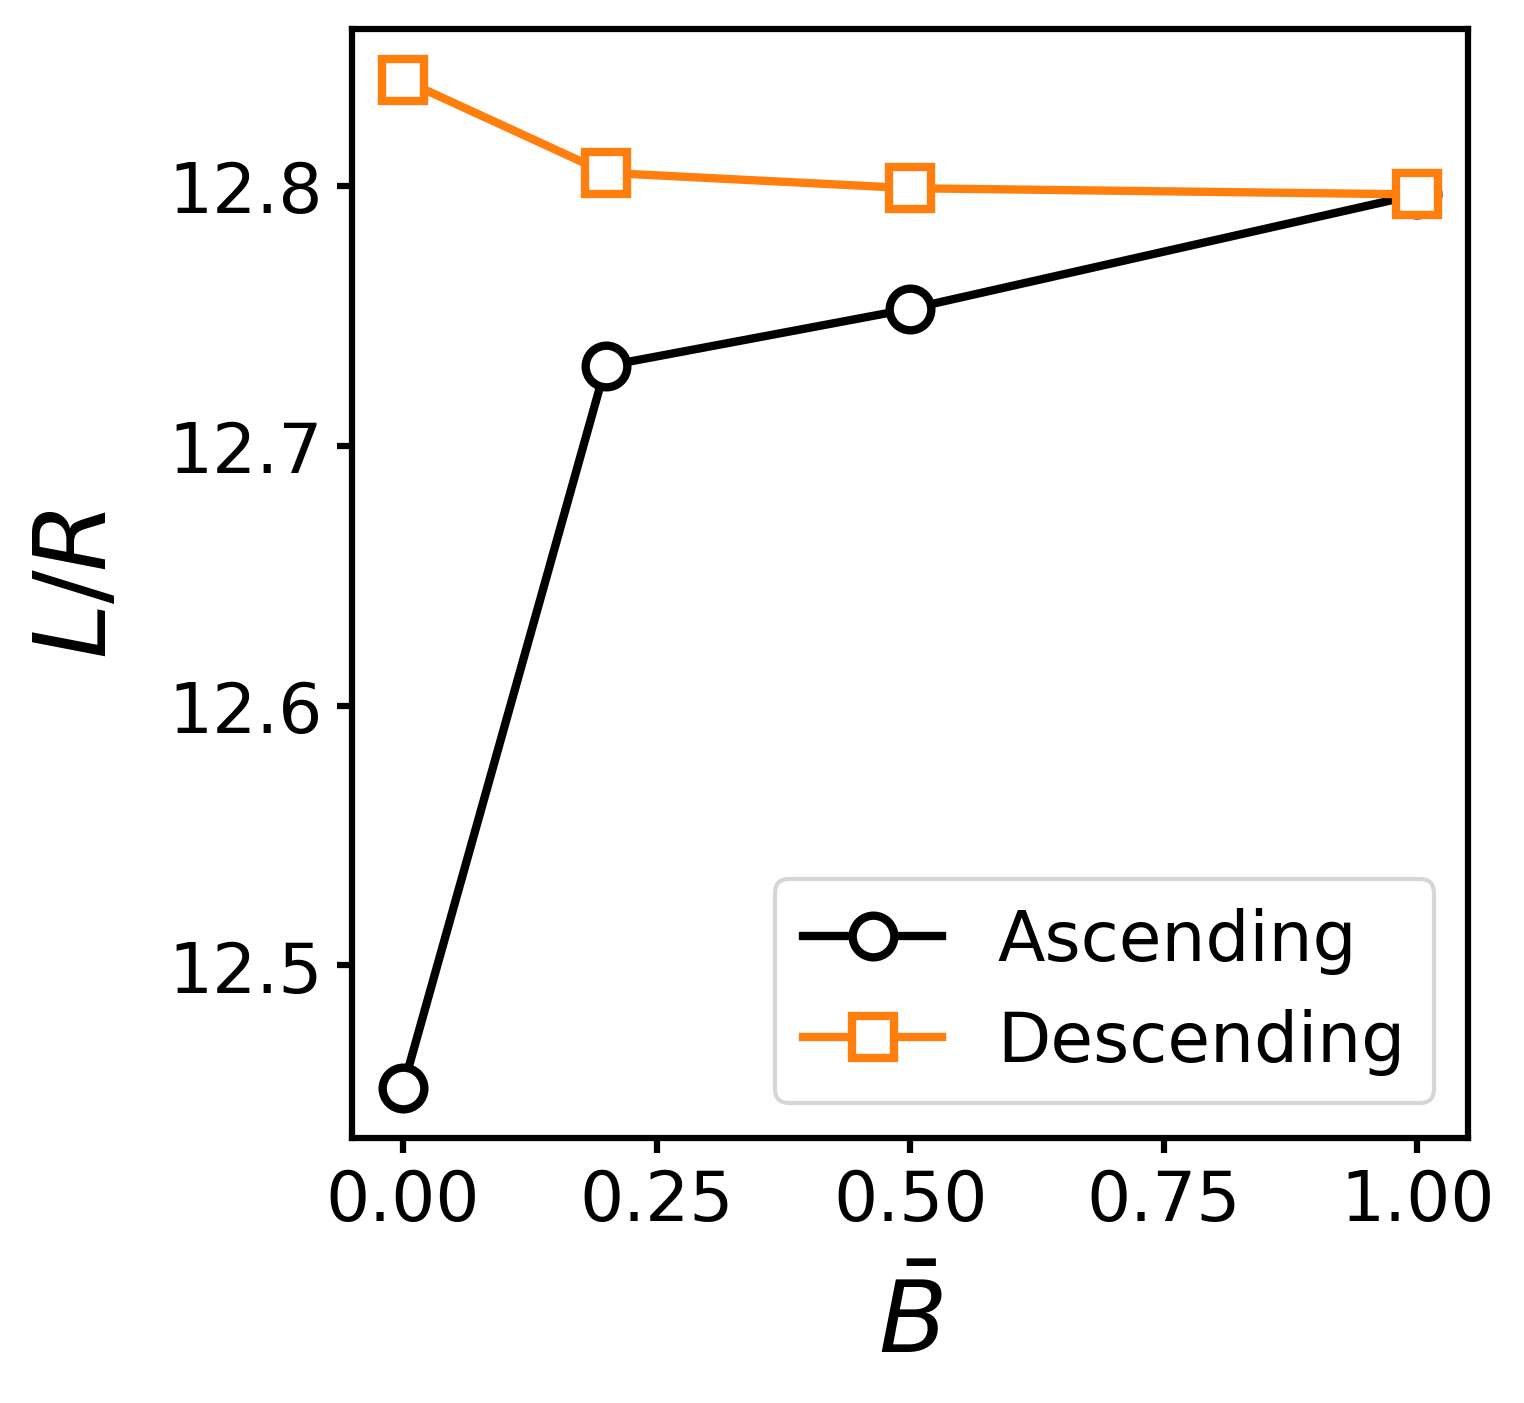
\includegraphics[scale=0.5]{../figures/results/paper2/hysteresis_curve.png} 
    \caption{Plot of the hysteresis curve of a bijel stabilized by magnetically responsive prolate particles. We observe that the domain size increases as we increase the applied
    magnetic field strength. However, upon decrease of the field strength, we see that the microstructure does not return to its previous value.} 
    \label{fig:hysteresis_curve} 
\end{figure}

Figure \ref{fig:hysteresis_curve} illustrates the hysteresis behavior of magnetically responsive bijels. We observe a hysteresis response of the 
bijel microstructure, characterized by a non-return of the microstructure to the original average domain size value when reducing the applied 
magnetic field strength. The increase in the average length scale when applying the magnetic field is due to domain coarsening caused by 
reorientation of particles to the magnetic field strength, reducing the interfacial coverage. When decreasing the magnetic field strength, 
we observe that the domain size does not return to the original value meaning that that the microstructure of the bijel is unaffected by 
the reduction in magnetic field. This suggests that the particles at the interface are in a kinetically trapped configuration.

\subsection{Field strength dependence on domain
size}\label{section:field-strength-dependence-on-domain-size}

Bijels have proposed applications as soft matter based material
templates, drug delivery vectors and separations systems. The materials
performance in each application is dependent upon the microstructure of
the bijel template. Many of the applications listed above benefit from
stimuli response, allowing for in-situ microstructure tuning to modify
permeability of the material. We want to understand whether bijels
provide access to reversible structural modifications which would allow
stimuli responsive bijels to be used in in-situ applications.
Additionally, in many of the proposed stimuli responsive applications
for bijels, the timescales of response is important to characterize and
would also provide a mechanistic understanding of the reasons why the
microstructure changes occur. We probe these aspects of structural
response of bijels in this section by assessing the response of bijels
stabilized by particles with volume fraction of \(\phi_p = 0.1\)
simulated under no applied field to an applied field in the range
\(\bar{B} = 0, 0.2, 0.5, 1\). We begin our investigation by visualizing
the structure before and after the application of magnetic fields.

\begin{figure} 
\centering 
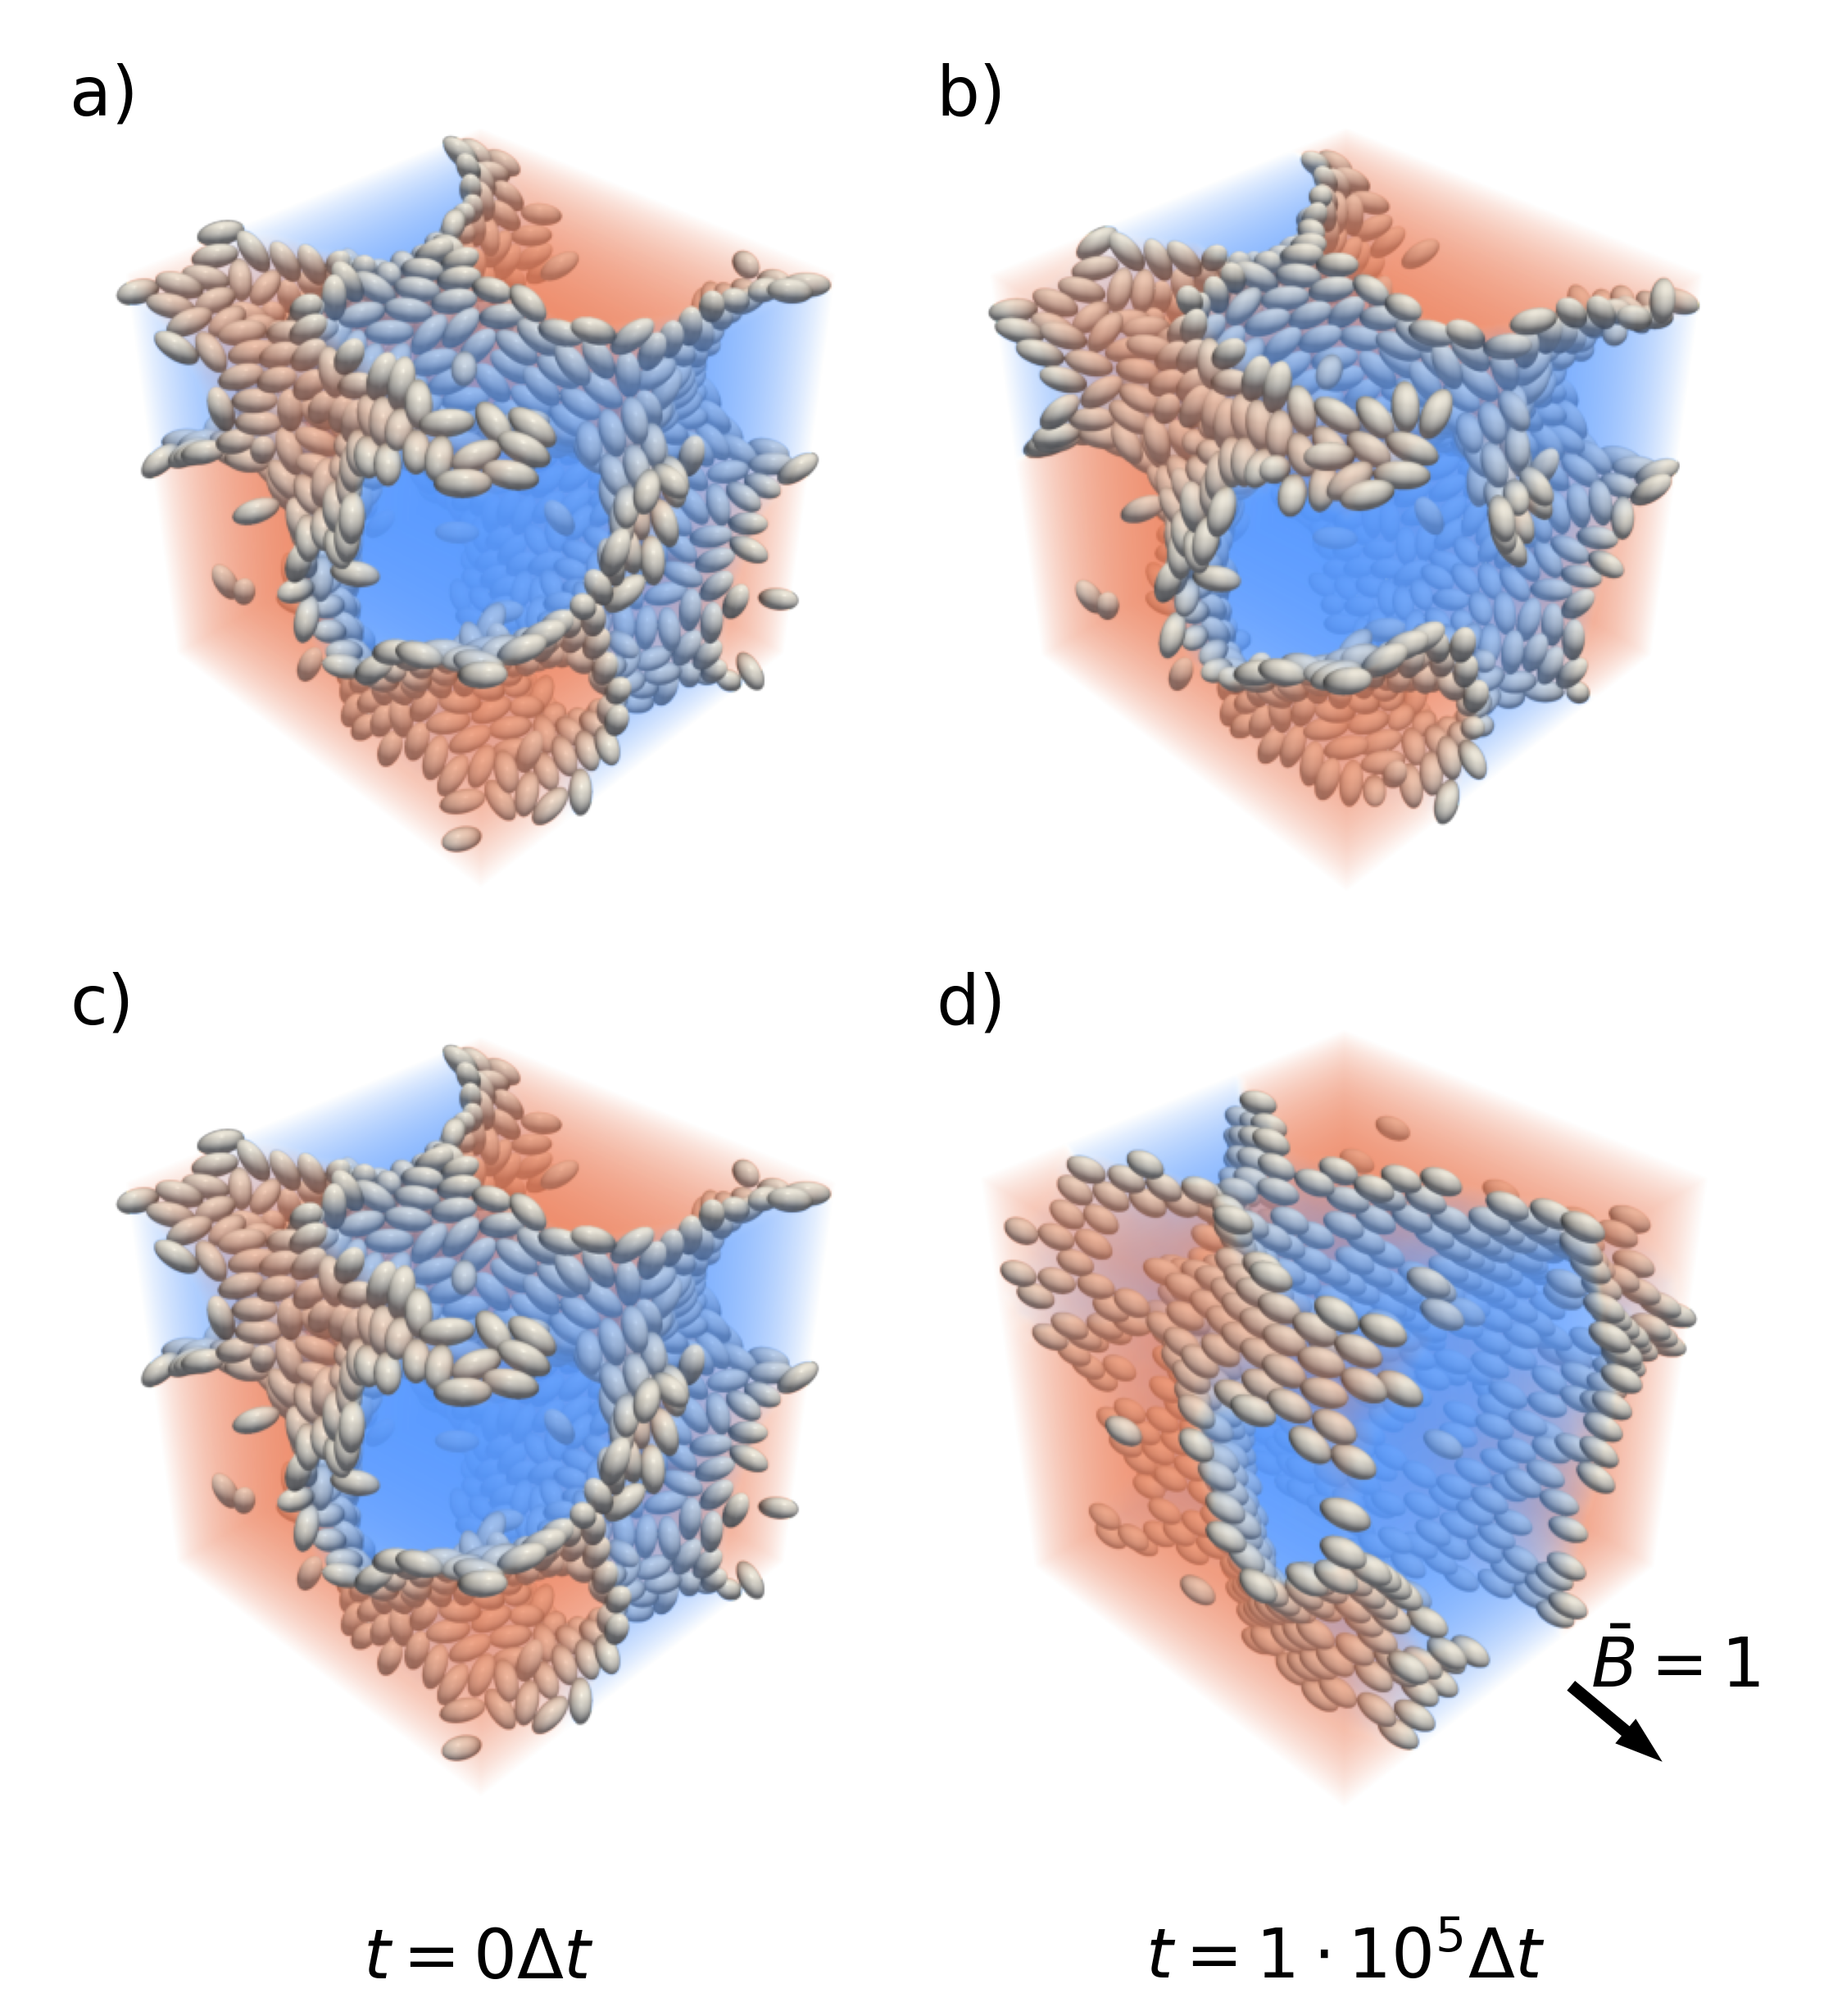
\includegraphics[scale=0.4]{../figures/results/paper2/microstructure_viz-field_on.png} 
\caption{Visualizations of bijels stabilized by oblate and prolate particles simulated under no fields at $t = 0$ (left columns) and $t = 10^5$ (right columns). The first and third row detail the microstructure evolution for oblate and prolate particle stabilized bijels with no applied field while the second and fourth rows show bijels stabilized by oblate and prolate particles respectively with a field strength of $\bar{B} = 1$ applied. Particle reorientation to the direction of the field can be seen upon application of the magnetic field, resulting in microstructure changes driven through domain coarsening until the particles jam. We see similar behavior in bijels stabilized by oblate particles upon application of the magnetic field.}
\label{fig:microstructure_viz-field_on} 
\end{figure}

In Figure \ref{fig:microstructure_viz-field_on} we show representative
snapshots of the bijel at the initial and final timestep with
\(\bar{B}_z = 0\) and \(\bar{B}_z = 1\). We show that upon application
of the field, particles align to the direction of the field. As the
particles orient to the field, they disrupt the packing of particles at
the interface, causing domain coarsening as the particles rearrange into
new positions. The particles then rejam in place once the interfacial
area and particle cross sectional area match. Domain coarsening observed
in the figure can be explained through the ordering of particles at the
interface, causing a reduction in the available area that the particles
have for stabilization.

To correlate the microstructure evolution to the ordering of the
particle monolayer to the magnetic field, we calculate the nematic order
parameter. \cite{veerman_phase_1992}

\begin{figure} 
\centering 
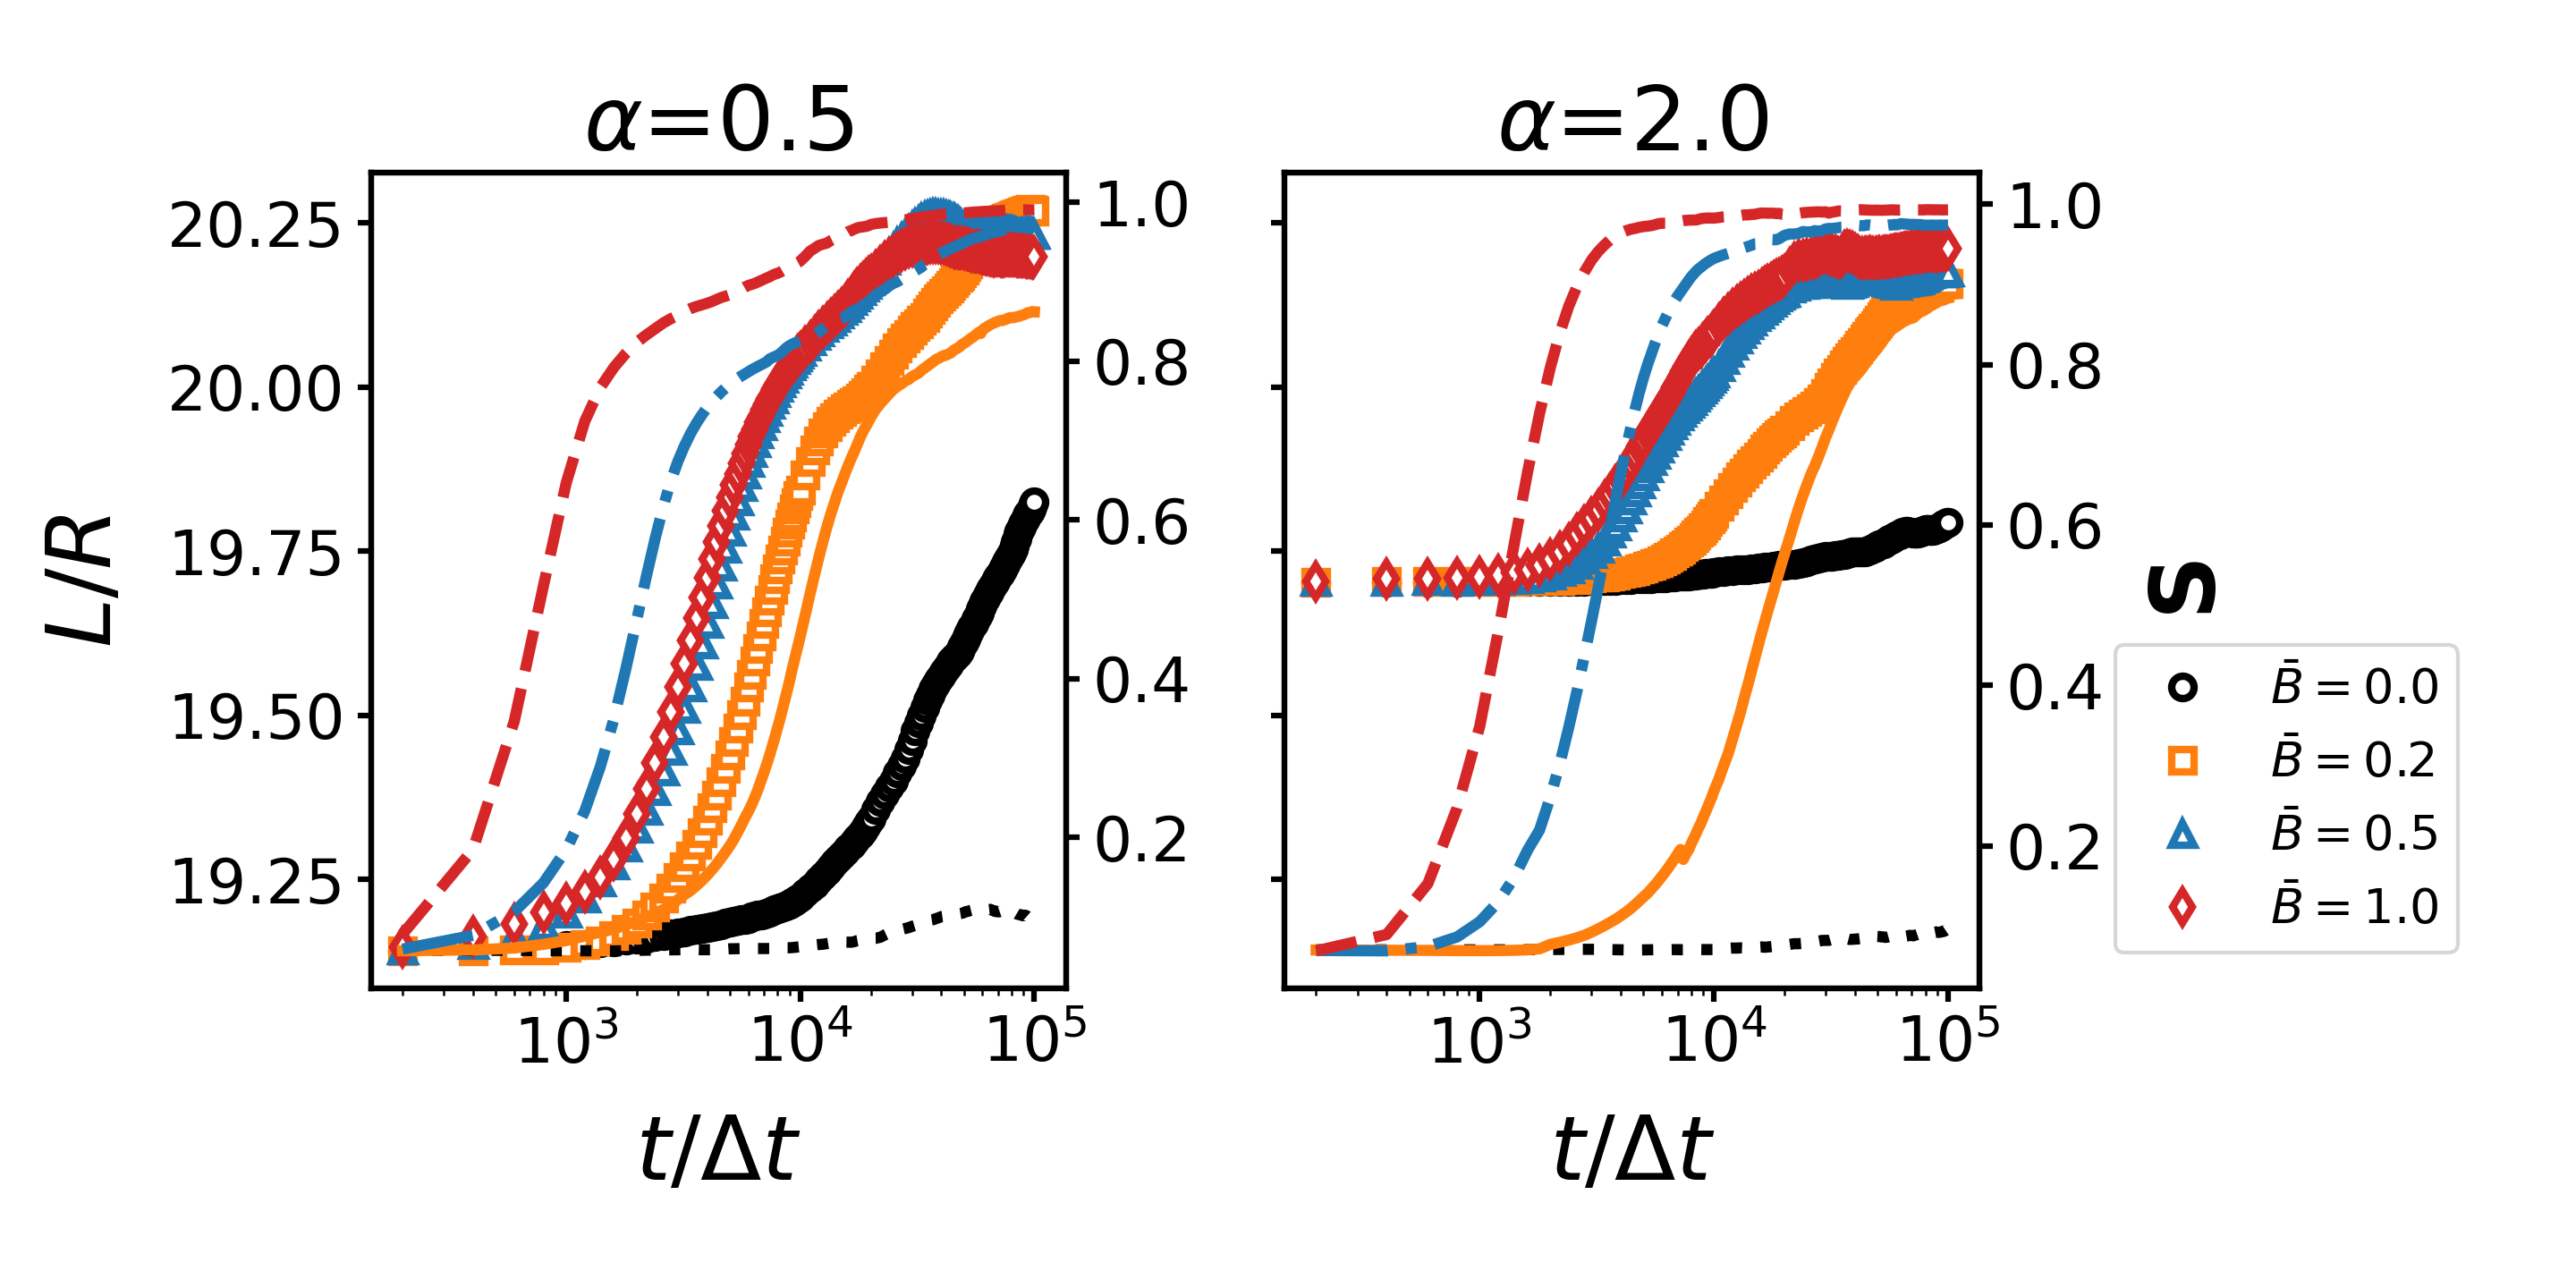
\includegraphics[scale=0.5]{../figures/results/paper2/domain_size-field_on.png} 
\caption{Plotting the spherically averaged domain size normalized with $R_p$($L/R$) of the particle at different magnetic field strengths, $\bar{B}$, and the nematic order parameter $S$ in lines. We quantify the domain size and ordering of the particles, and show that the change in both parameters are correlated with the strength of the applied magnetic field.} 
\label{fig:domain_size-field_on} 
\end{figure}

In Figure \ref{fig:domain_size-field_on}, we present the time evolution
of the normalized average domain size, where normalization is performed
using the volume-equivalent spherical particle radius \(R = 7.9\). The
results indicate that upon applying a magnetic field to a bijel
initially formed without one, the final average domain size increases by
up to 5.2\% and 2.5\% for oblate- and prolate-particle-stabilized bijels
respectively. Additionally, in the absence of an external field, domain
coarsening occurs for both particle morphologies. However, the results
for oblate particles with a magnetic field is attributed to coalescence
of domains rather than magnetic field driven ordering of the particles.

In the same figure, the time evolution of the nematic order parameter
\(S\) is also plotted to illustrate changes in particle alignment.
Initially, at \(\bar{B}_z = 0\), a gradual increase in \(S\) is
observed, attributed to steric interactions driving particle reordering.
This effect contributes to the domain coarsening seen in the absence of
an applied field, consistent with the findings of Günther et
al.~\cite{gunther_timescales_2014}. In the case of
oblate-particle-stabilized bijels without an external field, domain
coalescence is primarily driven by steric interactions rather than
field-induced rearrangement. Furthermore, the rate and extent of
particle alignment to the field exhibit a dependence on field strength,
as evidenced by the earlier onset of nematic ordering with increasing
\(\bar{B}\). We also observed between the time evolution of the nematic
order parameter and domain size, particularly when comparing results for
\(\bar{B}_z = 0.5, 1\) against those for \(\bar{B}_z = 0.2\). This
suggests that nematic ordering alone may not fully account for the
observed changes in domain size.

Previous studies have demonstrated that microstructural properties,
particularly length scale and tortuosity, play an important role in the
performance of porous materials across various applications, including
battery electrodes and tissue engineering. \cite{zhang_promoting_2019}
\cite{ebner_tortuosity_2014} \cite{hsieh_architected_2021} Specifically,
lower tortuosity and more ordered ion-conducting domains have been shown
to enhance charge/discharge rates in battery systems, while controlled
tortuosity in artificial bone grafts facilitates improved cell growth
and nutrient transport.

Precise characterization of the anisotropic microstructure is essential
for the tailored design of application-specific porous materials. To
quantify the characteristic length scales in each Cartesian direction,
we compute the second-moment-derived structure factor without radial
averaging. \cite{jansen_bijels_2011} We also calculate the tortuosity 
in each cartesian direction. Here, we make a further
refinement simplifying the domain sizes to directions parallel and
orthogonal to the magnetic field. These result in the length scales and
their associated calculation, \(L_{\parallel} = L_{z}\) and
\(L_{\perp} = \frac{L_x + L_y}{2}\). We perform the same simplification
with the directional tortuosities.

Tortuosity has been defined using
the geometric, diffusional and hydraulic tortuosities. Here we define
the diffusional tortuosity, \(\tau = \frac{D}{D_{eff}}\) which
characterizes the ratio between the free diffusion of a tracer and the
effective diffusion of a tracer in the material. Therefore, we plot
the directional second moment derived length scales and tortuosity in
Figure \ref{fig:domain_size_aniso-field_on}.

\begin{figure} 
\centering 
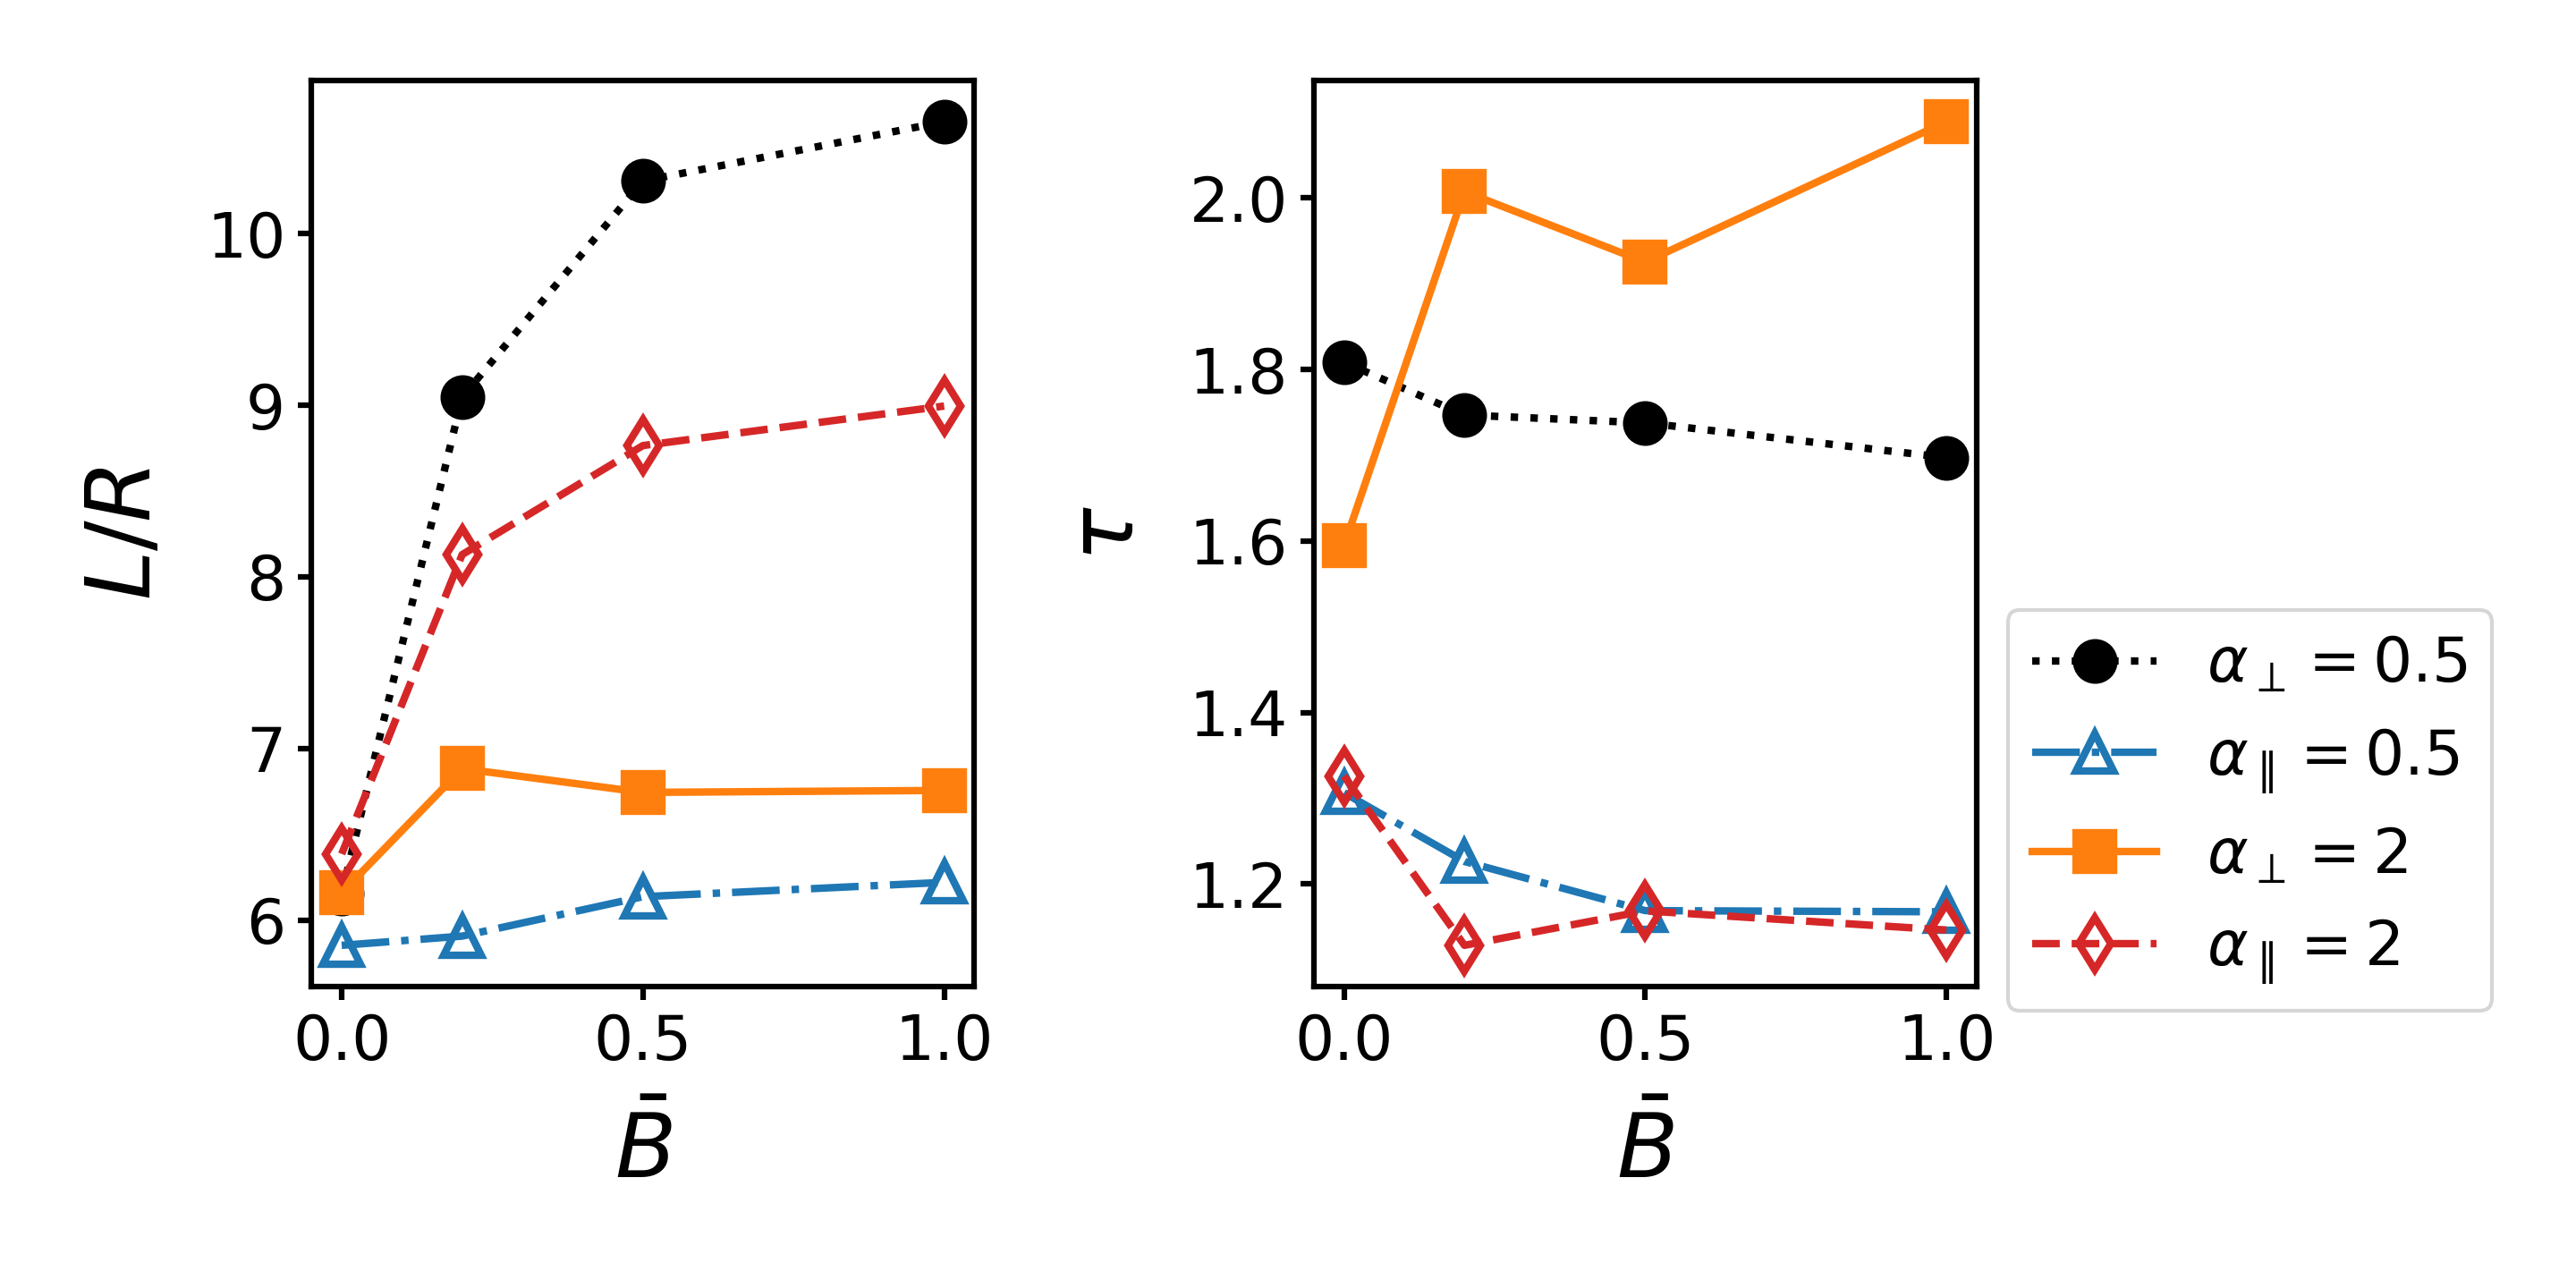
\includegraphics[scale=0.5]{../figures/results/paper2/domain_size_aniso-field_on.png} 
\caption{Plotting the anisotropic domain size and tortuosities against the applied magnetic field strength on the left and right respectively for bijels stabilized with magnetically responsive oblate and prolate ellipsoids. We see that upon application of the field, bijels stabilized with prolate particles experience a domains ize increase in the direction parallel to the applied field direction, $L_{\parallel}$, while the domain size perpendicular to the applied field, $L_{\perp}$ decreases. The opposite is true for bijels stabilized with oblate particles. The tortuosity data demonstrate that as the domain size increases, the tortuosity decreases and vice versa.} 
\label{fig:domain_size_aniso-field_on} 
\end{figure}

From Figure \ref{fig:domain_size_aniso-field_on}, we see that domain
size anisotropy is observed upon application of the field for both
particle morphologies. We also see some domain anisotropy with no
applied field, which increases upon application of the magnetic field.
The directional domain sizes, \(L_{\perp}\) and \(L_{\parallel}\)
increase by \(73\%\) and \(7\%\) respectively for oblate particles and
\(10\%\) and \(44\%\) respectively for oblate particles. The axes that
coarsens the most is consistent with past work, explained through the
directions particles reorient in response to the applied magnetic field.
As particles unjam and rejam at the interface due to reorientating to
the magnetic field, they adopt direction specific surface coverages
which manifest as anistropic domains upon jamming. In Figure
\ref{fig:domain_size_aniso-field_on}, we demonstrate that the
application of the magnetic field changes the domain size. The
tortuosity of the bijel is initially around \(\tau \approx 1.5\),
consistent with simulations of the diffusive tortuosities of gyroid
structures using Lattice Boltzmann simulations.
\cite{luo_macroscopic_2020} Upon application of the field,
\(\tau_{\perp}\) slightly decreases while \(\tau_{\parallel}\)
increases. We have seen that an increasing domain size decreases the
tortuosity in our past work. \cite{karthikeyan_formation_2024} This
observation is in line with the domain size changes observed in Figure
\ref{fig:domain_size_aniso-field_on}. The results show that the
tortuosity of the bijel is noticeably affected by the application of
magnetic fields. This data suggests that magnetic fields applied onto
bijels stabilized with ellipsoidal particles undergo domain anisotropy
upon application of magnetic fields. However the particle morphology,
specifically its axis of symmetry, affect the direction that the domain
anisotropy is characterized.

Next, we turn to investigate the time gap between the average domain
size increase and the nematic order parameter. We hypothesized that the
time taken for particle reorientation to the field would control the
degree and rate of domain size change when the bijel begins with
particles with random order. This result suggests that the dynamics of
the system at higher magnetic field strengths are dependent upon other
factors that vary upon application of the magnetic field. To understand
this phenomena, we focus on the dynamics of the particle monolayer.
First, we visualize the particle monolayer of the bijels stabilized with
prolate ellipsoids at the initial and final configuration before and
after application of a magnetic field.

\begin{figure} 
\centering 
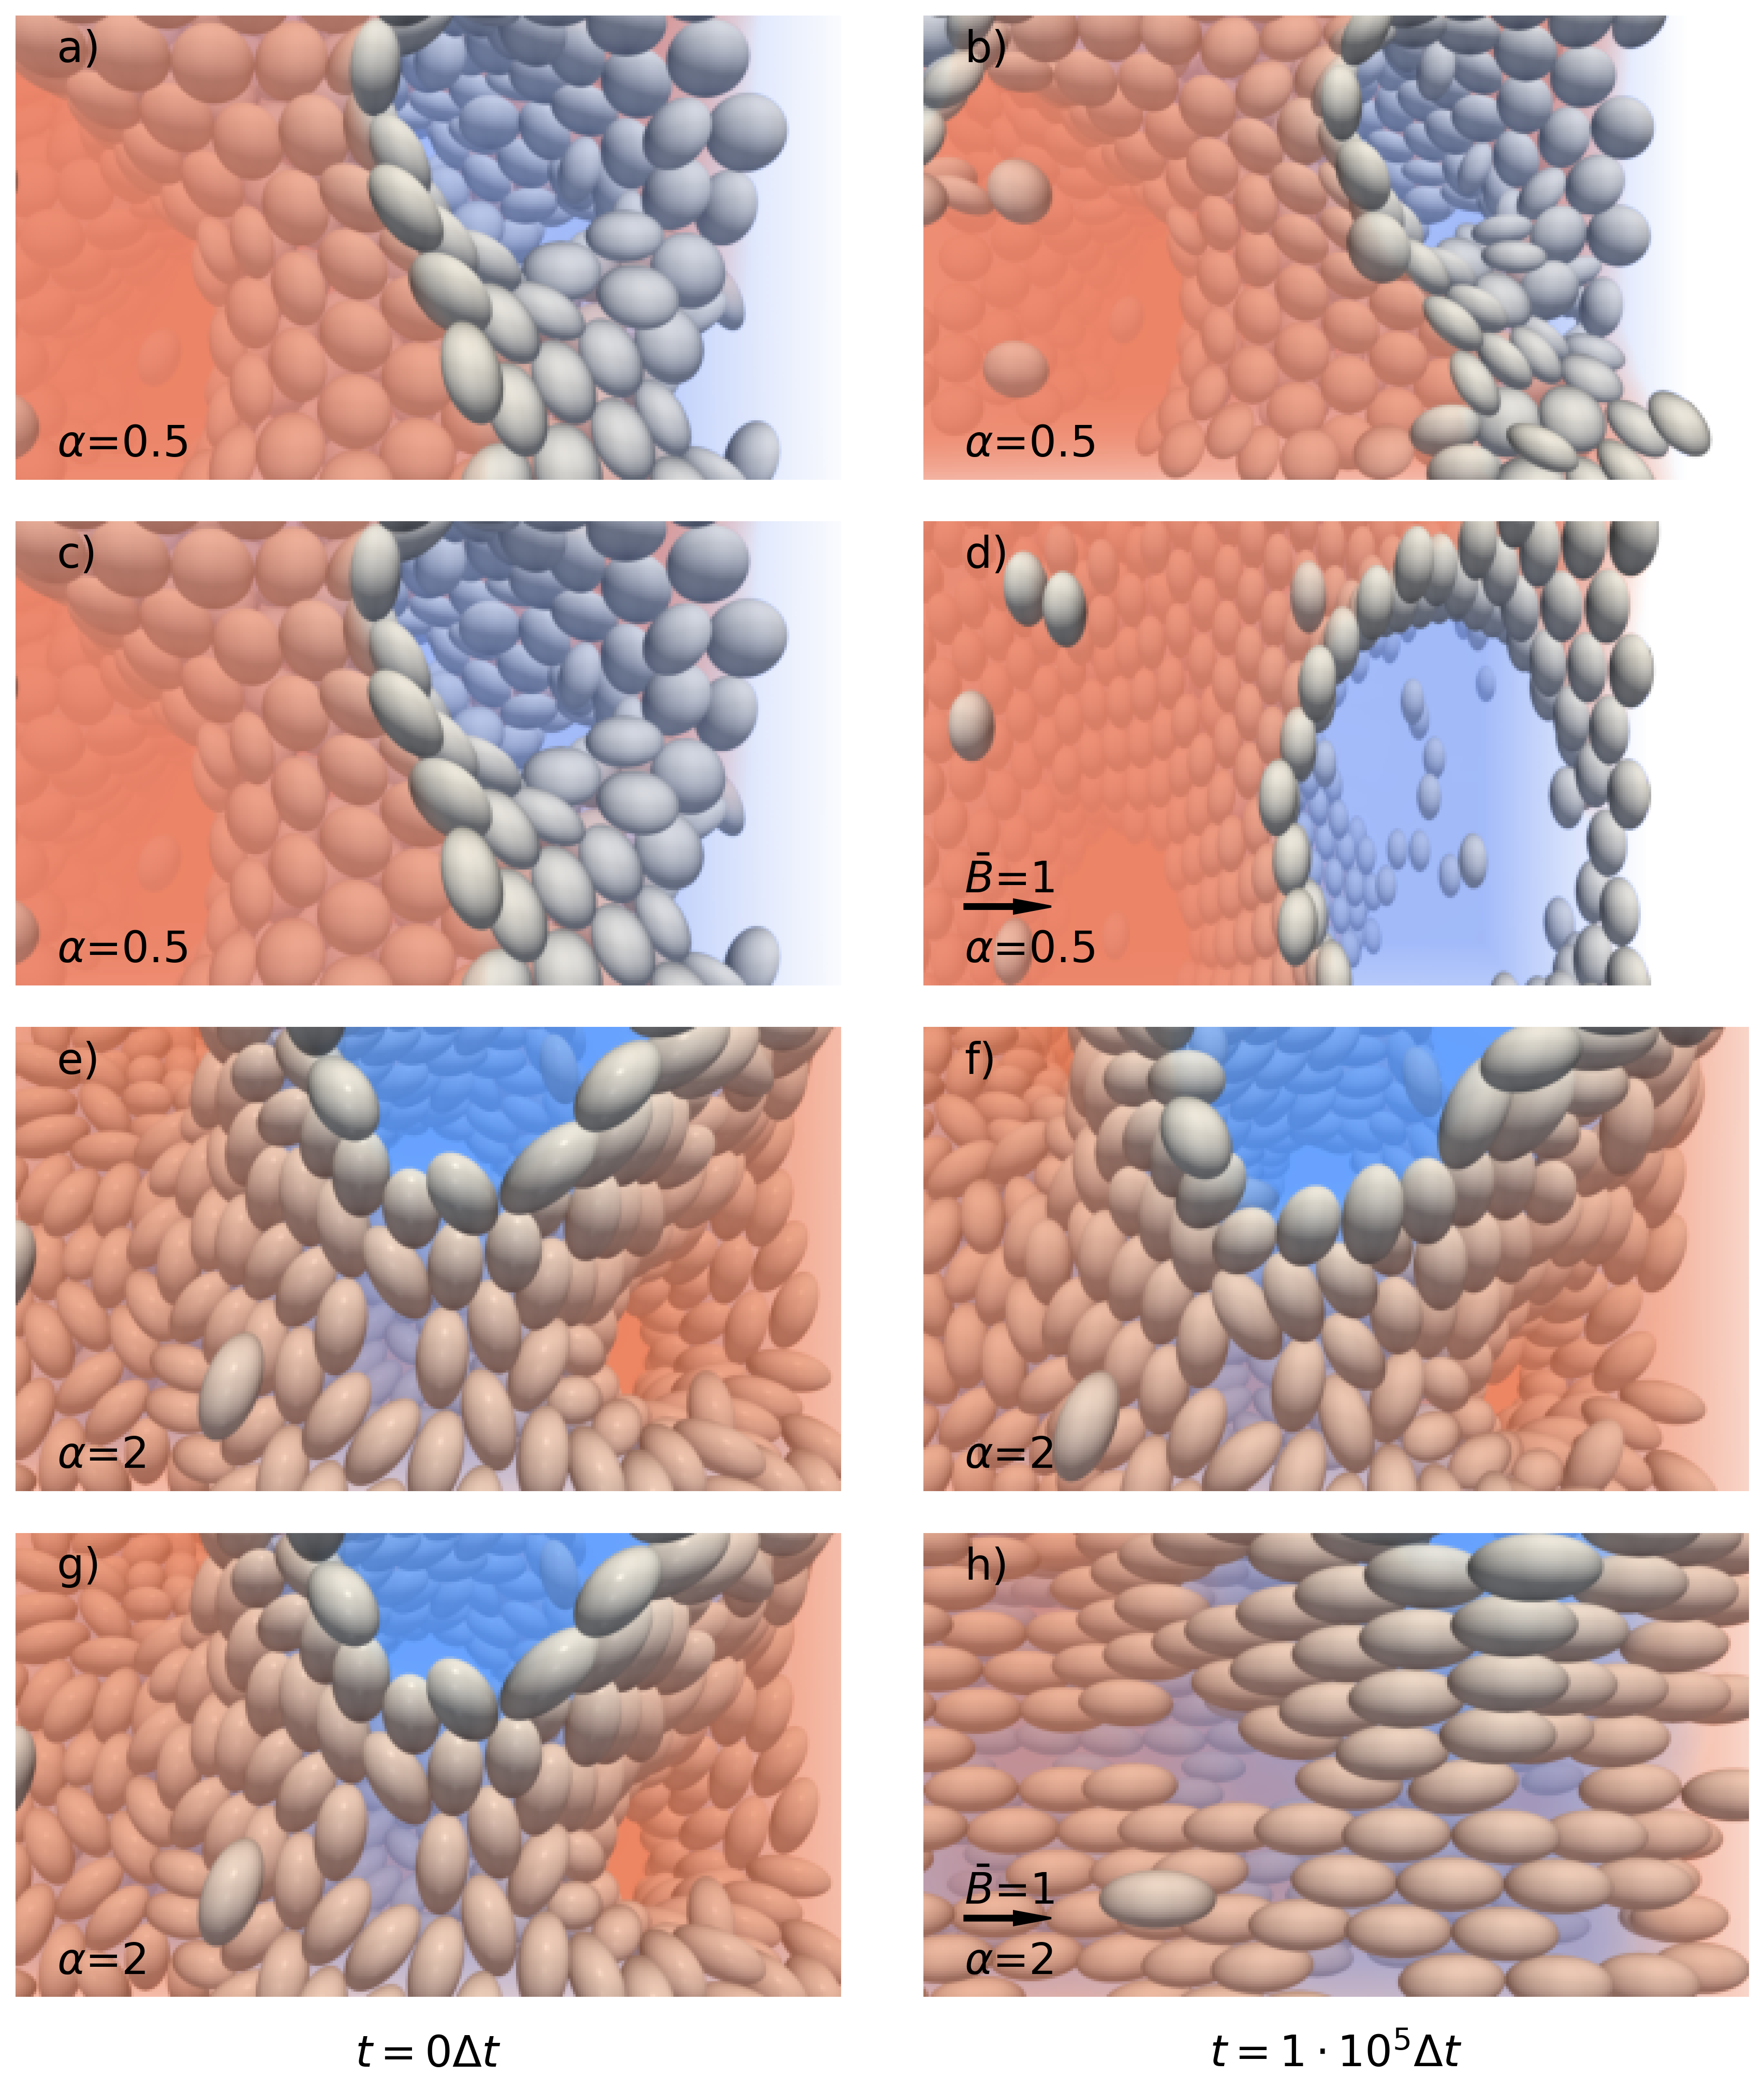
\includegraphics[scale=0.2]{../figures/results/paper2/particle_viz-field_on.png} 
\caption{Visualizations of bijels stabilized with oblate and prolate particles simulated at $t = 0$ (left column) and $t = 10^5$ (right column). The first and third rows show the particle monolayer of bijels stabilized with oblate and prolate ellipsoids respectively with no applied field. The second and fourth rows show the particle monolayer of bijels stabilized with oblate and prolate ellipsoids respectively with an applied field of $\bar{B}_z = 1$. Particle reorientation to the direction of the field can be seen, resulting in coarsening of the domains.} 
\label{fig:particle_viz-field_on} 
\end{figure}

In Figure \ref{fig:particle_viz-field_on}, we see the effect of the
application of the magnetic field on the monolayer. The initial
configuration of particles at the monolayer show that the orientations
are random and that the particles tend to lie flat on the interface.
However, upon application of the magnetic field the particles orient to
the field direction. The effect that Gunther. et al.~observed for bijels
stabilized with anisotropic particles can also be observed in these
snapshots as the particles can be observed to have more local order in
the final state than in the initial state with no applied field. We
observe that for bijels stabilized by prolate ellipsoids, we see the
adoption of more regular arrangements of the colloids on the interface.
We investigate the effect of local particle ordering next. Past work by
Bresme and Faraudo and Davies investigating the reorientation of
particles at interfaces under magnetic fields have shown that a critical
magnetic field exists, above which the particle orients to the field and
below which the particle orientation is a function of the capillary
force and magnetic field derived force. \cite{davies_interface_2014}
\cite{bresme_orientational_2007} Particle adsorption into the interface
with microparticles have also been shown to be irreversible due to the
high adsorption energy. Upon particle reorientation, the microstructure
change can be driven solely through particle unjamming and re-jamming,
or it can be driven through the particles dragging the interface during
this process. The mechanism of unjamming and re-jamming can be
investigated using the average interfacial angle, $\langle \psi \rangle$
and the local ordering of the particles characterized with 
$\langle Q_6 \rangle$ Past work has identified that local crystallization 
of colloidal crystals takes place at \(\langle Q_6 \rangle = 0.38\). 
\cite{toxvaerd_role_2020}

\begin{figure} 
\centering 
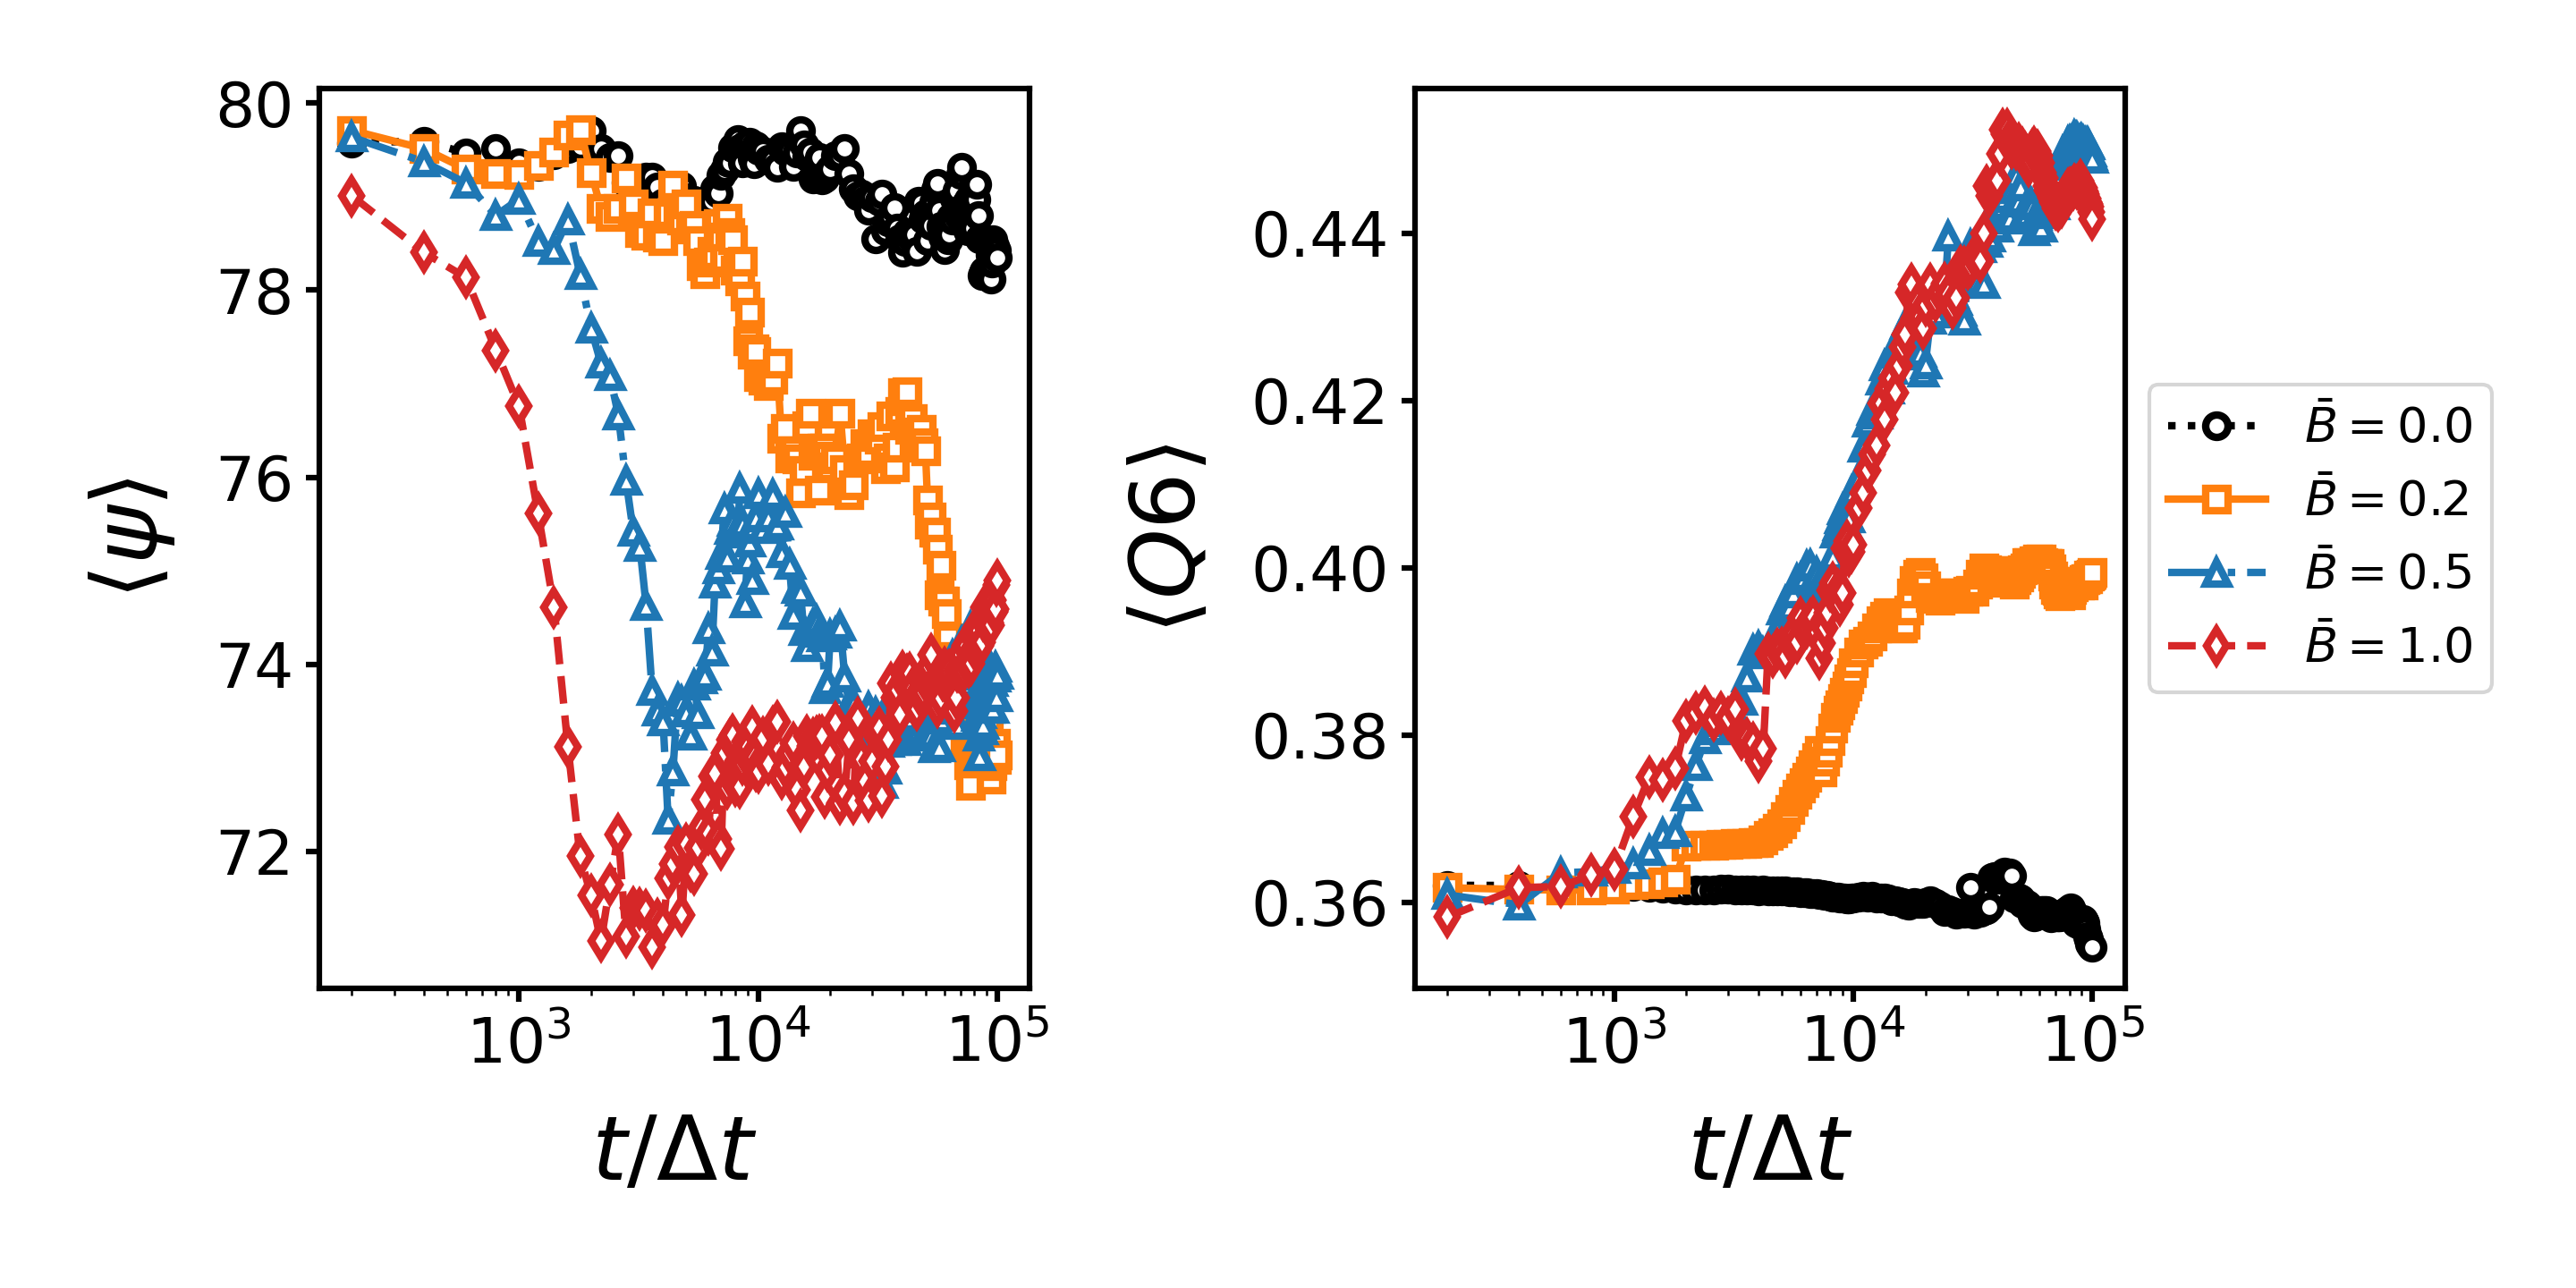
\includegraphics[scale=0.5]{../figures/results/paper2/interface_angle-nint-field_on.png} 
\caption{Plots of the interface angle $(\langle \psi \rangle)$ and six fold Steinhardt order parameter $(\langle Q_6 \rangle)$ on the left and right respectively, versus time for bijels stabilized with oblate and prolate ellipsoids on the top and bottom rows respectively. We demonstrate that upon application of a magnetic field, the behavior of $(\langle \psi \rangle)$ and $(\langle Q_6 \rangle)$ differ significantly between oblate and prolate ellipsoids indicating that the dynamics for both particle morphologies differ. We also observe magnetic field dependence in each property for both particle types, suggesting that these changes are driven primarily through the change in the applied field strength.} 
\label{fig:interface_angle-nint-field_on} 
\end{figure}

From Figure \ref{fig:interface_angle-nint-field_on}, we identify that
prolate and oblate particles respond differently at the interface. For
bijels stabilized by oblate ellipsoids, we characterize an increase in
\(\langle \psi \rangle\) from an initial value of \(19 ^{\circ}\),
before it reduces slightly and begins to increase once again. The
initial starting value of \(\langle \psi \rangle\) indicates the
particles are lying close to flat on the interface, before they begin to
tilt out of the interface when the magnetic field is applied. Then,
\(\langle \psi \rangle\) plateaus as the interface begins to move in
response to the tilting particle at the interface. This is caused by the
large adsorption energy of the particles at the interface of the bijel,
caused by high surface tension. Finally, the particles jam in place,
locking the interface at an angle to the particle. We see the rate of
increase in \(\langle \psi \rangle\) at early stages and the time spent
in the plateau increase with a larger applied magnetic field. The final
angle at the interface is also dependent upon the applied field
strength.

When analyzing \(\langle \psi \rangle\) for bijels stabilized by prolate
particles, this behavior can also be observed. \(\langle \psi \rangle\)
begins at \(80 ^{circ}\). The difference in the initial
\(\langle \psi \rangle\) compared to oblate particles is due to the
direction of the axis of symmetry. In prolate particles, the axis of
symmetry lies parallel with the interface and \(\langle \psi \rangle\)
measures the angle between the interface normal and the orientation of
the axis of symmetry. We see \(\langle \psi \rangle\) decrease slightly,
before plateauing and slowly increasing again. The rate of decrease in
\(\langle \psi \rangle\) is field dependent, although given the small
decrease in \(\langle \psi \rangle\) it is unclear if the final value of
this parameter is field dependent for bijels stabilized with prolate
particles. The changes in \(\langle \psi \rangle\) for bijels stabilized
with prolate particles are small compared to bijels stabilized with
oblate particles. We believe this is due to local particle effects at
the interface. We probe this by identifying the local particle ordering
at the interface characterized by \(\langle Q_6 \rangle\).

We see that for oblate particles, \(\langle Q_6 \rangle\) sees a
decrease from its initial value. However the dynamics are controlled by
the applied magnetic field strength. We split the phases of dynamics
into three sections, similar to \(\langle \psi \rangle\) with the first
section seeing a decrease in \(\langle Q_6 \rangle\) upon application of
the magnetic field, followed by a plateau and finally a gradual increase
before jamming takes place. These results indicate that the ordering of
the particles is reduced by the applied magnetic field, before a
restoration of some of the pre-existing order. The final values of
\(\langle Q_6 \rangle\) are magnetic field dependent, with a stronger
magnetic field having a lower final \(\langle Q_6 \rangle\) value
indicating that either the ordering of particles influence the angle at
the interface or vice versa. We observe that for bijels stabilized by
oblate particles, the interface ordering of the particles increases as a
function of the applied field strength. We also observe from plotting
\(\langle Q_6 \rangle\) that application of a magnetic field creates a
local crystallization of the colloid monolayer characterized as
\(\langle Q_6 \rangle > 0.38\). \cite{toxvaerd_role_2020}

Figure \ref{fig:domain_size-field_on}, we observed a gap between the
growth of the nematic order parameter and an increase in the domain
size. To probe why this occurs, we recast \(\langle \psi \rangle\),
\(\langle Q_6 \rangle\) and \(S\) in terms of the physical phenomena
they represent. The nematic order parameter represents the ordering of
particles to an average direction, which in the case of the application
of a magnetic field, is the field direction. Therefore, a timescale
reliant on the nematic order parameter would represent a timescale of
response rate limited to the response to the magnetic field, which
indicates a particle-field orientation dependence. We name this
timescale \(\tau_S\). When applying a field to a bijel system with a
randomly oriented particle monolayer, the most significant transition
point is the isotropic to nematic transition or when \(S \geq 0.3\). We
define \(\tau_S\) for this section of the analysis by identifying when
\(S \geq 0.3\).

We can also do the same for \(\langle \psi \rangle\) and
\(\langle Q_6 \rangle\). A timescale derived from
\(\langle \psi \rangle\) named \(\tau_{\langle \psi \rangle}\)
represents the capillary timescale between the interface and the
particle. Given the shape of the plot, we assign the
\(\tau_{\langle \psi \rangle}\) to be the time when the first minimum of
\(\langle \psi \rangle\) is observed for prolate particles and the first
maximum for oblate particles. A timescale derived from
\(\langle Q_6 \rangle\), named \(\tau_{\langle Q_6 \rangle}\) is also
calculated which represents a timescale of local particle rearrangement.
We define \(\tau_{\langle Q_6 \rangle}\) as the time when
\(\langle Q_6 \rangle \geq 0.38\) for prolate particles and the global
minimum of \(\tau_{\langle Q_6 \rangle}\) for the oblate particles. We
omit \(\bar{B} = 0\) as previous results have identified the domain size
changes observed there. We then plot the average domain size \(L\)
against time rescaled with these three timescales in Figure
\ref{fig:domain_size-field_on-scaled}.

\begin{figure} 
\centering 
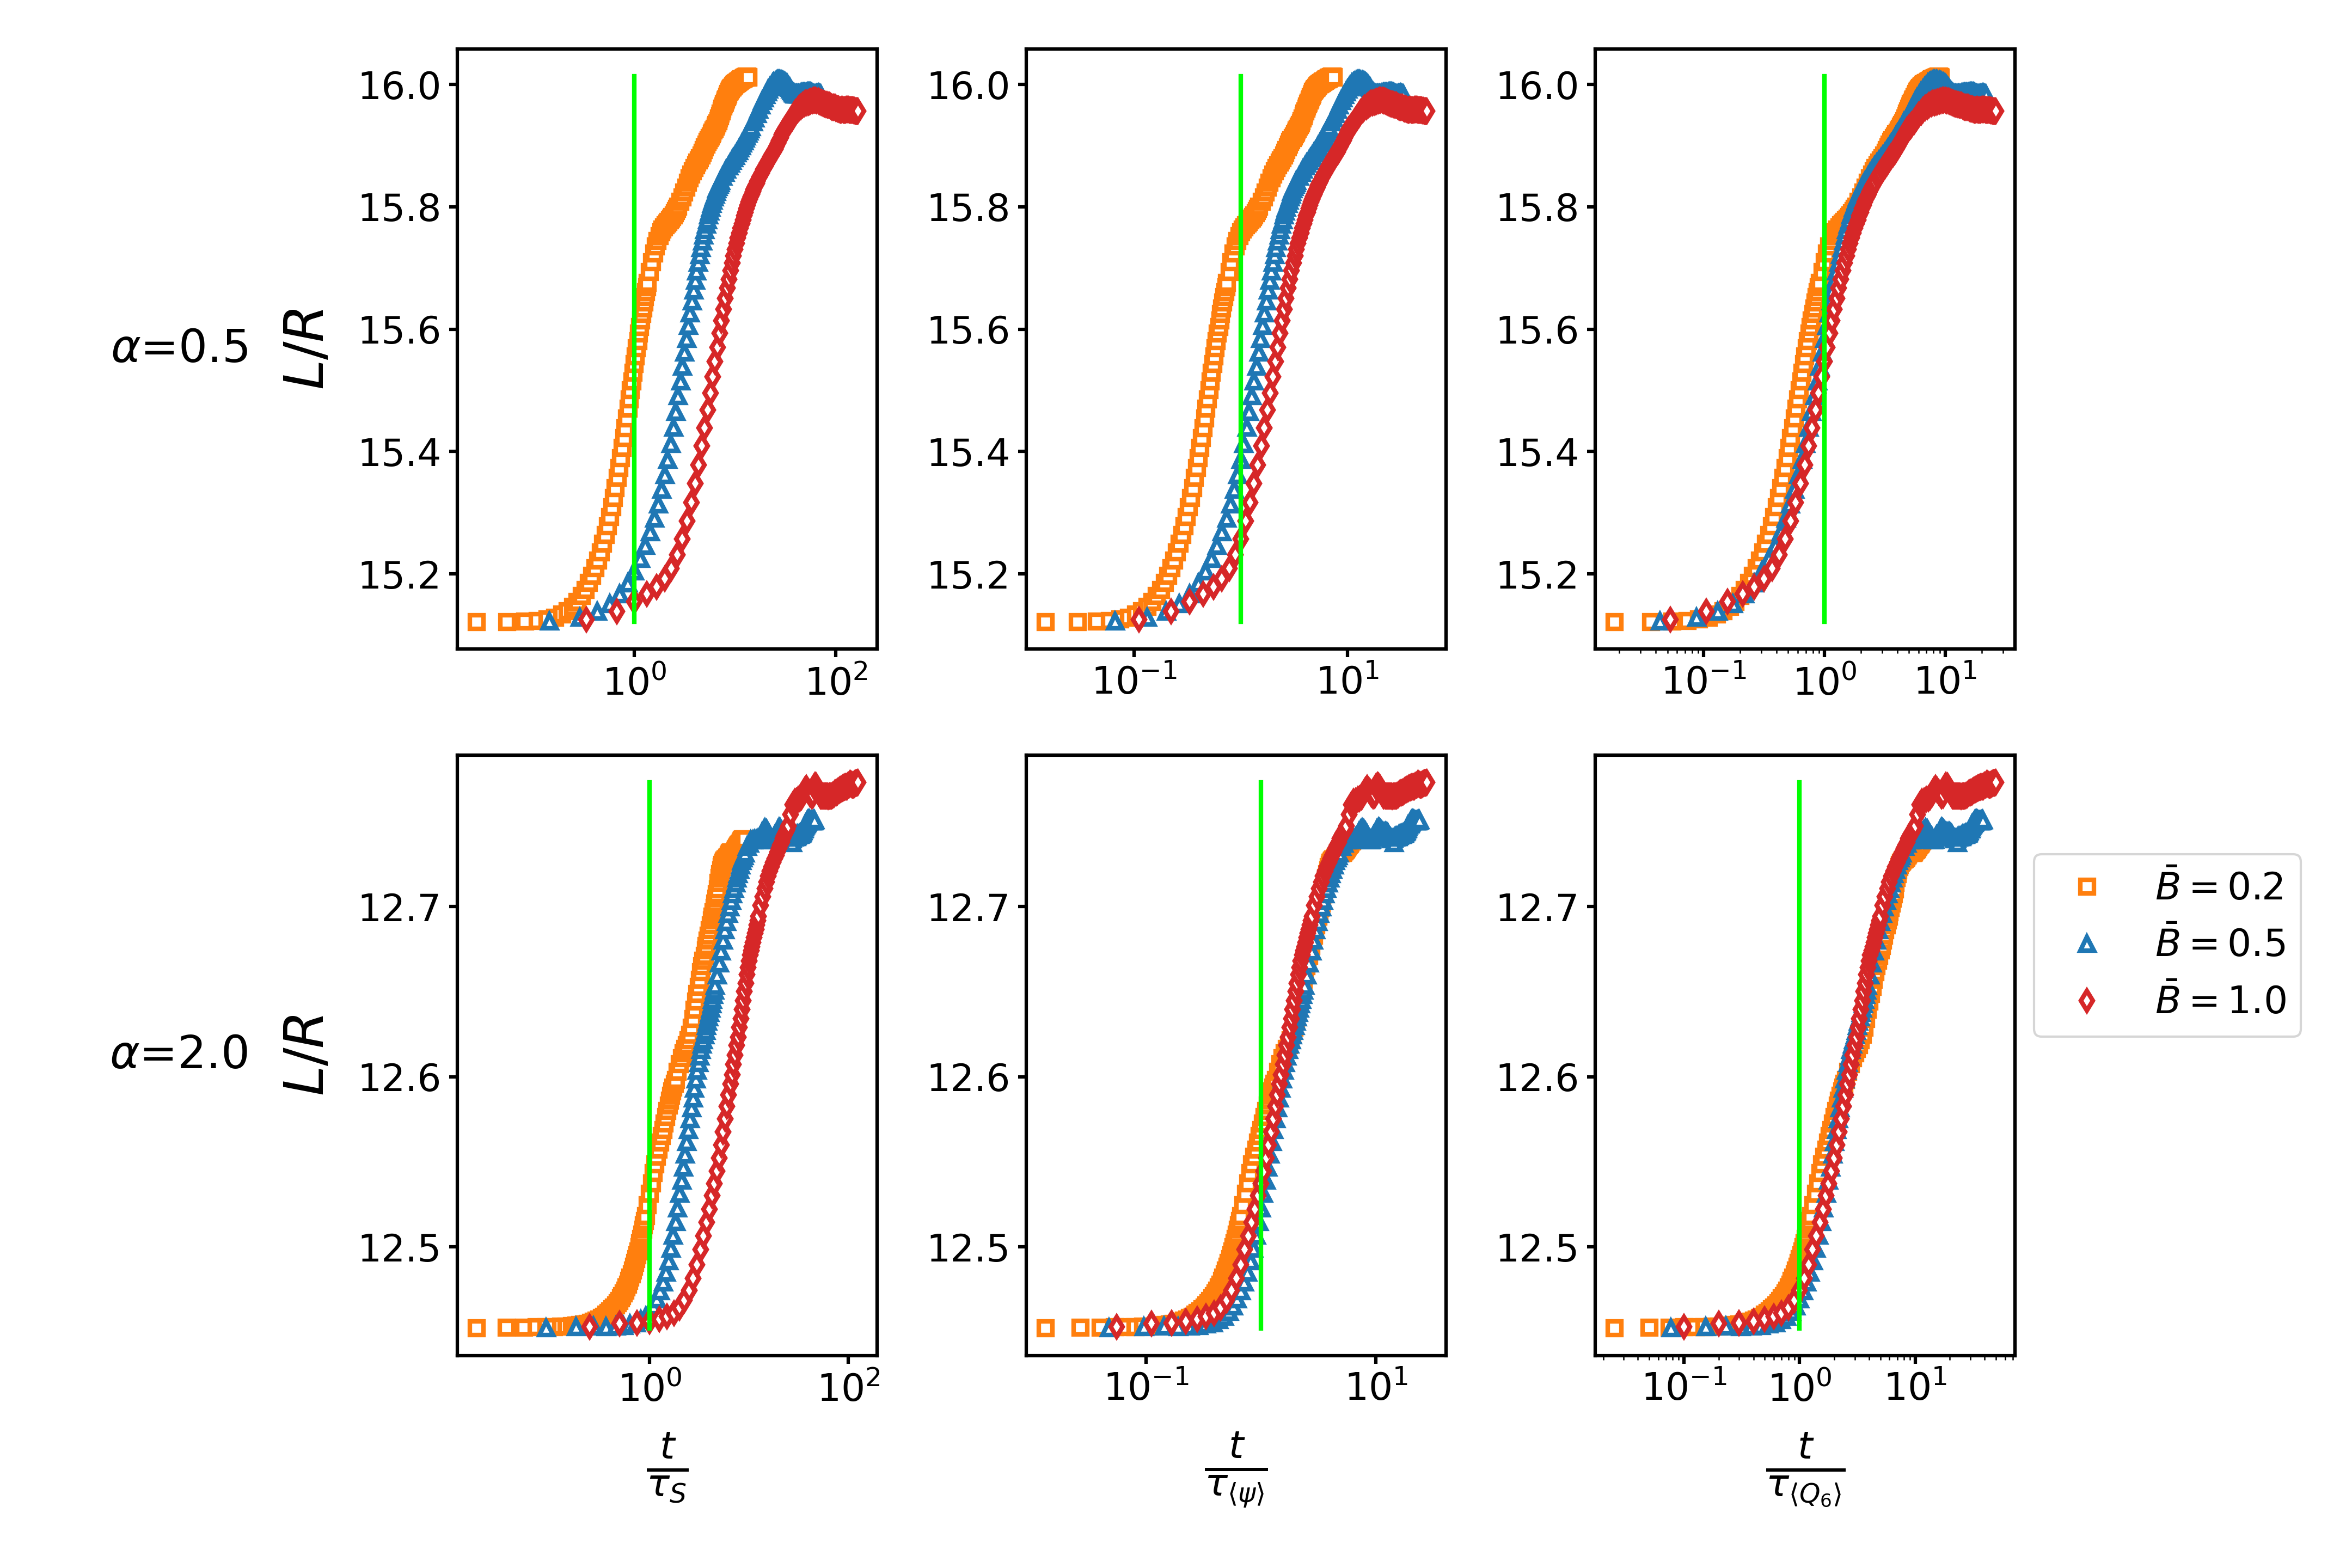
\includegraphics[scale=0.4]{../figures/results/paper2/domain_size-field_on-scaled.png} 
\caption{Plots of domain size with different timescales. The top and bottom row represent the average domain size for bijels stabilized with oblate and prolate particles respectively. The figures on the left plots the domain size against time rescaled with the nematic to isotropic transition time, $\tau_S$. The figures in the middle plot the domain size against time rescaled with the interfacial capillary timescale, $\tau_{\langle \psi \rangle}$. The figures on the right plot the domain size against time rescaled with the particle rearrangement timescale, $\tau_{\langle Q_6 \rangle}$. We show that the controlling timescale when applying a magnetic field onto bijels with disordered particles is the latter timescale, indicating that the dominating effect is steric hindrance of the particles during rearrangment at the interface.} 
\label{fig:domain_size-field_on-scaled} 
\end{figure}

In Figure \ref{fig:domain_size-field_on-scaled}, the left plot plots the
average domain size against time rescaled using \(\tau_S\). We see that
the domain sizes do not collapse onto a single line, which is expected
if we want to explain the dynamics using the nematic order parameter.
This confirms the observation made above that the dynamics do not only
depend on the reorientation of particles to the field. The middle plot
demonstrates the average domain size against time rescaled using
\(\tau_{\langle \psi \rangle}\). We see that there is good agreement
between all simulations for prolate particles, although the point when
\(\frac{t}{\tau_{\langle \psi \rangle}} = 1\) lies when the domain size
transition has started. However for oblate particles we see that this
timescale does not describe the dynamics well.

The right plot demonstrates the domain size change after rescaling time
with \(\tau_{\langle Q_6 \rangle}\) where we see good collapse between
all plots while the domain size transition also begins at
\(\frac{t}{\tau_{\langle Q_6 \rangle}} = 1\). The latter point
demonstrates that the dynamics for the structural response of randomly
oriented particles are controlled by the local particle rearrangement at
the interface rather than the orientation of the particle to the
magnetic field.We see that before \(\tau_{\langle Q_6 \rangle} = 1\),
\(\bar{B} = 0.2\) for the oblate particles does not collapse onto the
other plots, indicating that the dynamics before that point are
controlled by another phenomena.

From the evidence in Figure \ref{fig:domain_size-field_on-scaled}, two
types of interfacial behaviors are characterized in addition to that
identified by Gunther et al.~\cite{gunther_timescales_2014} The first
type is what is observed for \(\bar{B} = 0.2\), where the interfacial
coverage and average orientation of the particle to the field and to the
interface change in lock step. This causes the interface to reorient at
the same rate as the particles reorienting to the magnetic field. The
second is observed for \(\bar{B} = 0.5, 1\), where there is a time lag
between particle ordering, and the intiation of domain coarsening. In
the latter scenario, at early times the particles are jolted out of
position before the large adsorption energy of the particles into the
interface causes the interface to move to the particle position, causing
domain coarsening as the interfacial area reduces.

\subsection{Increasing the applied
field}\label{increasing-the-applied-field}

We saw in the hysteresis curve that the microstructure change at higher
field strengths began to reduce with each subsequent field strength
jump, suggesting that the ordering of the particles were linked to the
domain size change observed. In the previous section, we saw that domain
size changes in bijels after jamming are constrained by magnetic field
driven local crystallization of the particle monolayer. In this section,
we explore how pre-existing order in the particles affect the degree of
domain size change observed. We apply fields of strength
\(\bar{B}_{template} = 0, 0.2, 0.5, 1\) during phase separation to
create bijels stabilized with ellipsoidal particles with pre-existing
particle order. We then apply a field strength of \(\bar{B}_z = 1\) and
observe the time evolution of the system for \(t = 10^5\) timesteps. We
simplify our nomenclature here demonstrated with an example.
\(\bar{B}_z: 0.0 \rightarrow 1.0\) represents a bijel made with no
field, and a field of \(\bar{B}_z = 1.0\) applied after the structure
has reached steady state. We begin by visualizing the microstructure
changes experienced by bijels simulated with pre-existing particle order
in Figure \ref{fig:microstructure_viz-field_up}.

\begin{figure}
\centering 
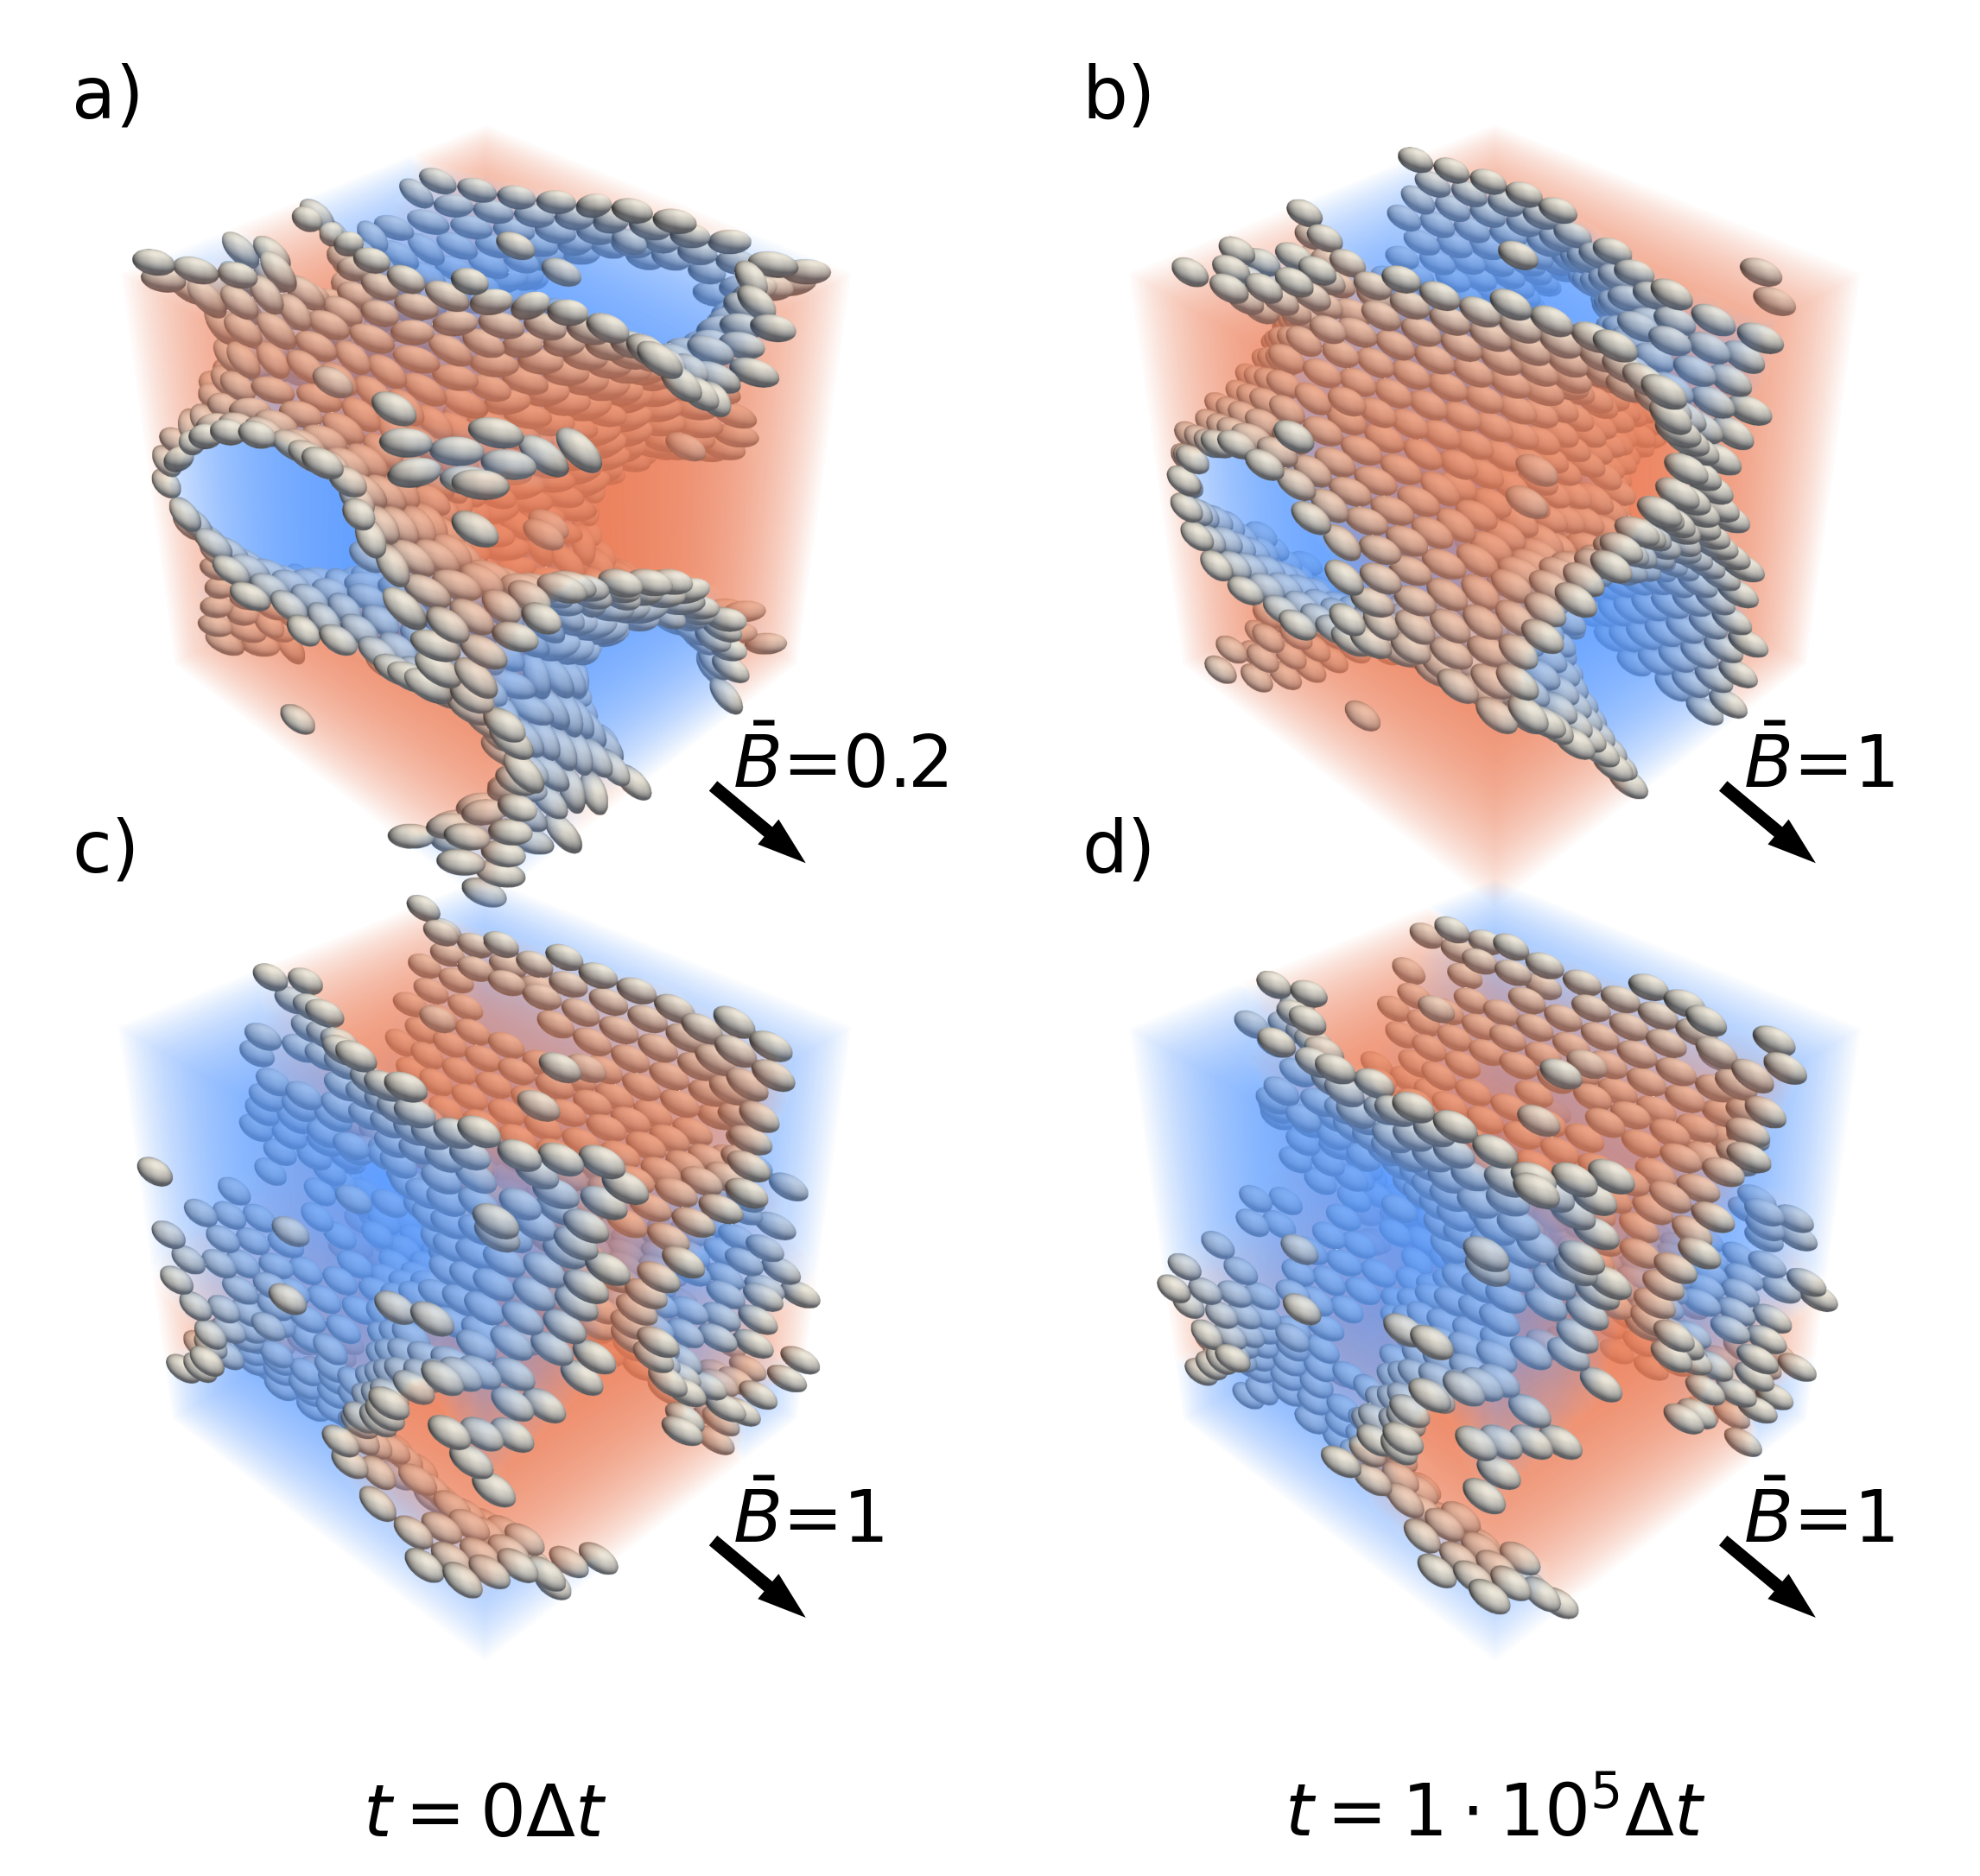
\includegraphics[scale=0.4]{../figures/results/paper2/microstructure_viz-field_up.png} 
\caption{Visualizations of bijels stabilized with oblate and prolate particles simulated at $t = 0$ (left column) and $t = 10^5$ (right column). The first and third rows show the particle monolayer of bijels stabilized with oblate and prolate ellipsoids respectively with an applied field of $\bar{B}_z = 0.2$. The second and fourth rows show the particle monolayer of bijels stabilized with oblate and prolate ellipsoids respectively with an applied field of $\bar{B}_z = 1$. We increase the applied field to $\bar{B}_z = 1$ in both cases and show that particle reorientation to the field occurs at the $\bar{B}_z = 0.2$ but not in the $\bar{B}_z = 1$ case.}
\label{fig:microstructure_viz-field_up}
\end{figure}

In Figure \ref{fig:microstructure_viz-field_up} we show representative
snapshots of a bijel stabilized with prolate particles at the initial
and final timestep with field conditions
\(\bar{B}_z: 0.2 \rightarrow 1.0\) and
\(\bar{B}_z: 1.0 \rightarrow 1.0\) in the top and bottom rows
respectively. We show that upon application of the field, the fluid
domains undergo a field strength dependent microstructrue response, with
the degree of response dependent upon the difference between the initial
and final magnetic field. We also observe a qualitative increase in the
alignment of the particles to the magnetic field for the
\(\bar{B}_z: 0.2 \rightarrow 1.0\) case. We quantify these observations
by plotting the average domain size and nematic order parameter in
Figure \ref{fig:domain_size-field_up}.

\begin{figure} 
\centering 
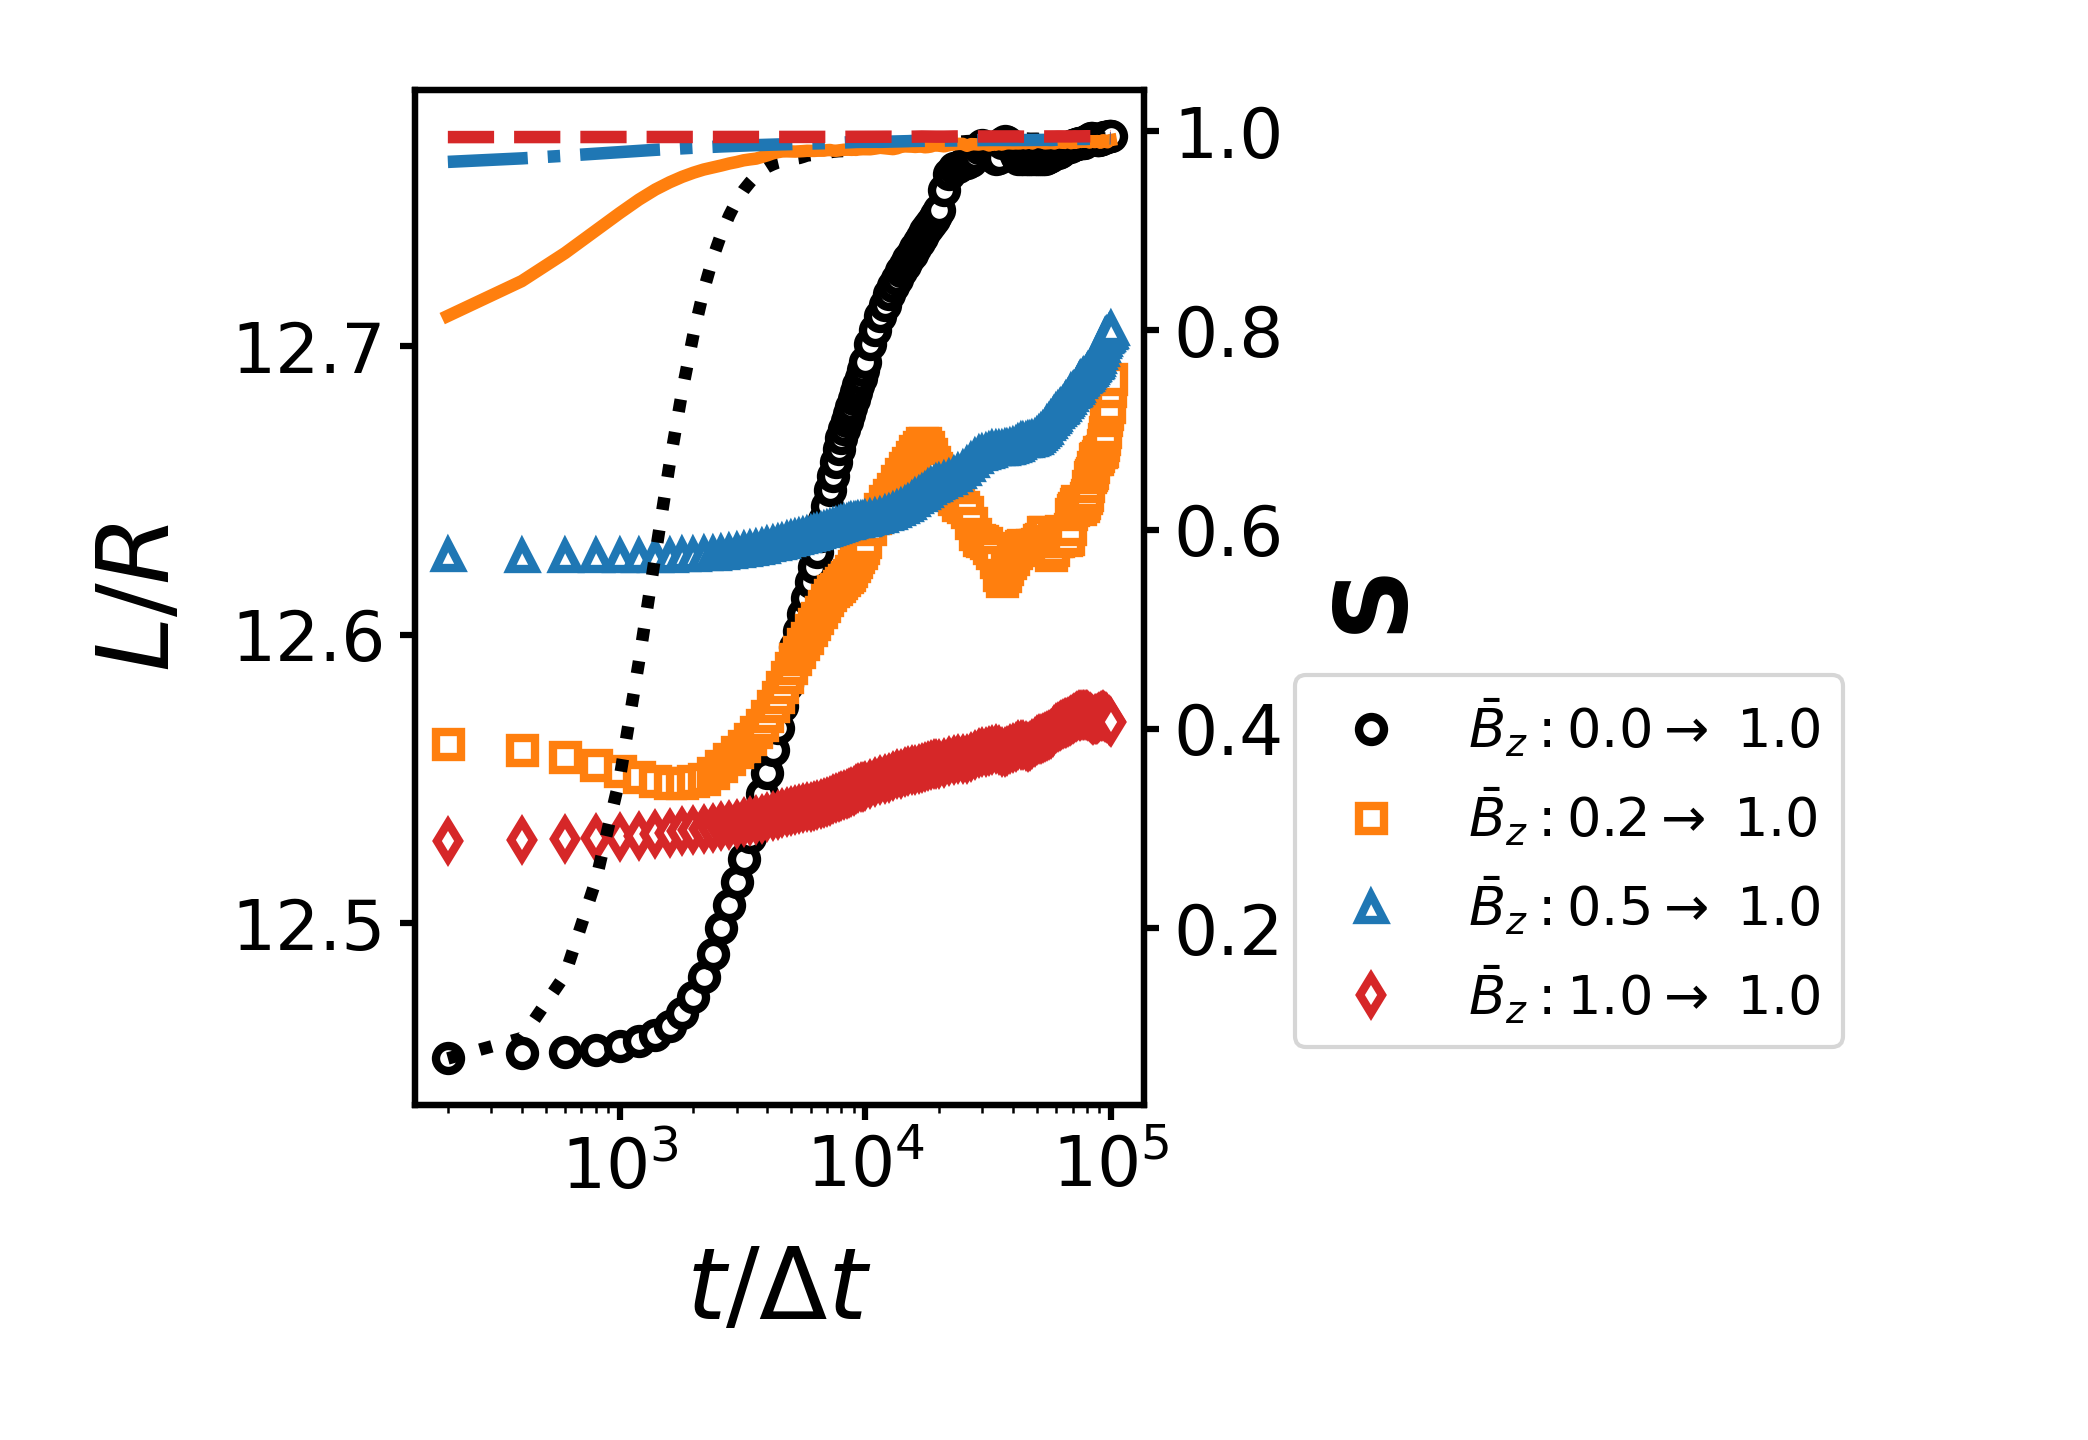
\includegraphics[scale=0.5]{../figures/results/paper2/domain_size-field_up.png} 
\caption{Plot of the spherically averaged domain size normalized with $Rp(L/R)$ of the particle in markers and the nematic order parameter in lines. We show that the domain size change measured is correlated to the change in the particle ordering, characterized using the nematic order parameter.} 
\label{fig:domain_size-field_up} 
\end{figure}

In Figure \ref{fig:domain_size-field_up}, we define the difference
between the final and initial magnetic field strengths as
\(\Delta \bar{B}\). The onset of microstructural response is observed to
be \(\Delta \bar{B}\)-dependent, indicating that a stronger driving
force is required to induce structural reorganization. Additionally, the
extent of microstructural change is also correlated with
\(\Delta \bar{B}\), where \(\Delta \bar{B} = 1\) results in average
microstructural variations of 5\% and 2\% for oblate and prolate
particles, respectively which decreases as \(\Delta \bar{B}\) decreases.
We further characterize the relationship between \(\Delta \bar{B}\) and
nematic order, showing that an increase in \(S\) correlates with
\(\Delta \bar{B}\). This suggests that changes in domain size are
intrinsically linked to the initial particle ordering within the system.
These findings indicate that characteristic length scale evolution is
dependent on both aspect ratio and field strength variation,
highlighting the role of particle alignment in governing domain
coarsening dynamics. To further quantify the anisotropic microstructural
evolution, we define the relative change in domain size as
\(\Delta L = \frac{L_{f} - L_{i}}{L_{i}}\), where \(L\) represents
either \(L_{\perp}\) or \(L_{\parallel}\). The same formulation is
applied to the tortuosity in the respective directional components. We
do this to characterize the \(\Delta \bar{B}\)-dependent changes
observed in the domain anisotropy. The results are presented in Figure
\ref{fig:domain_size_aniso-field_up}.

\begin{figure} 
\centering 
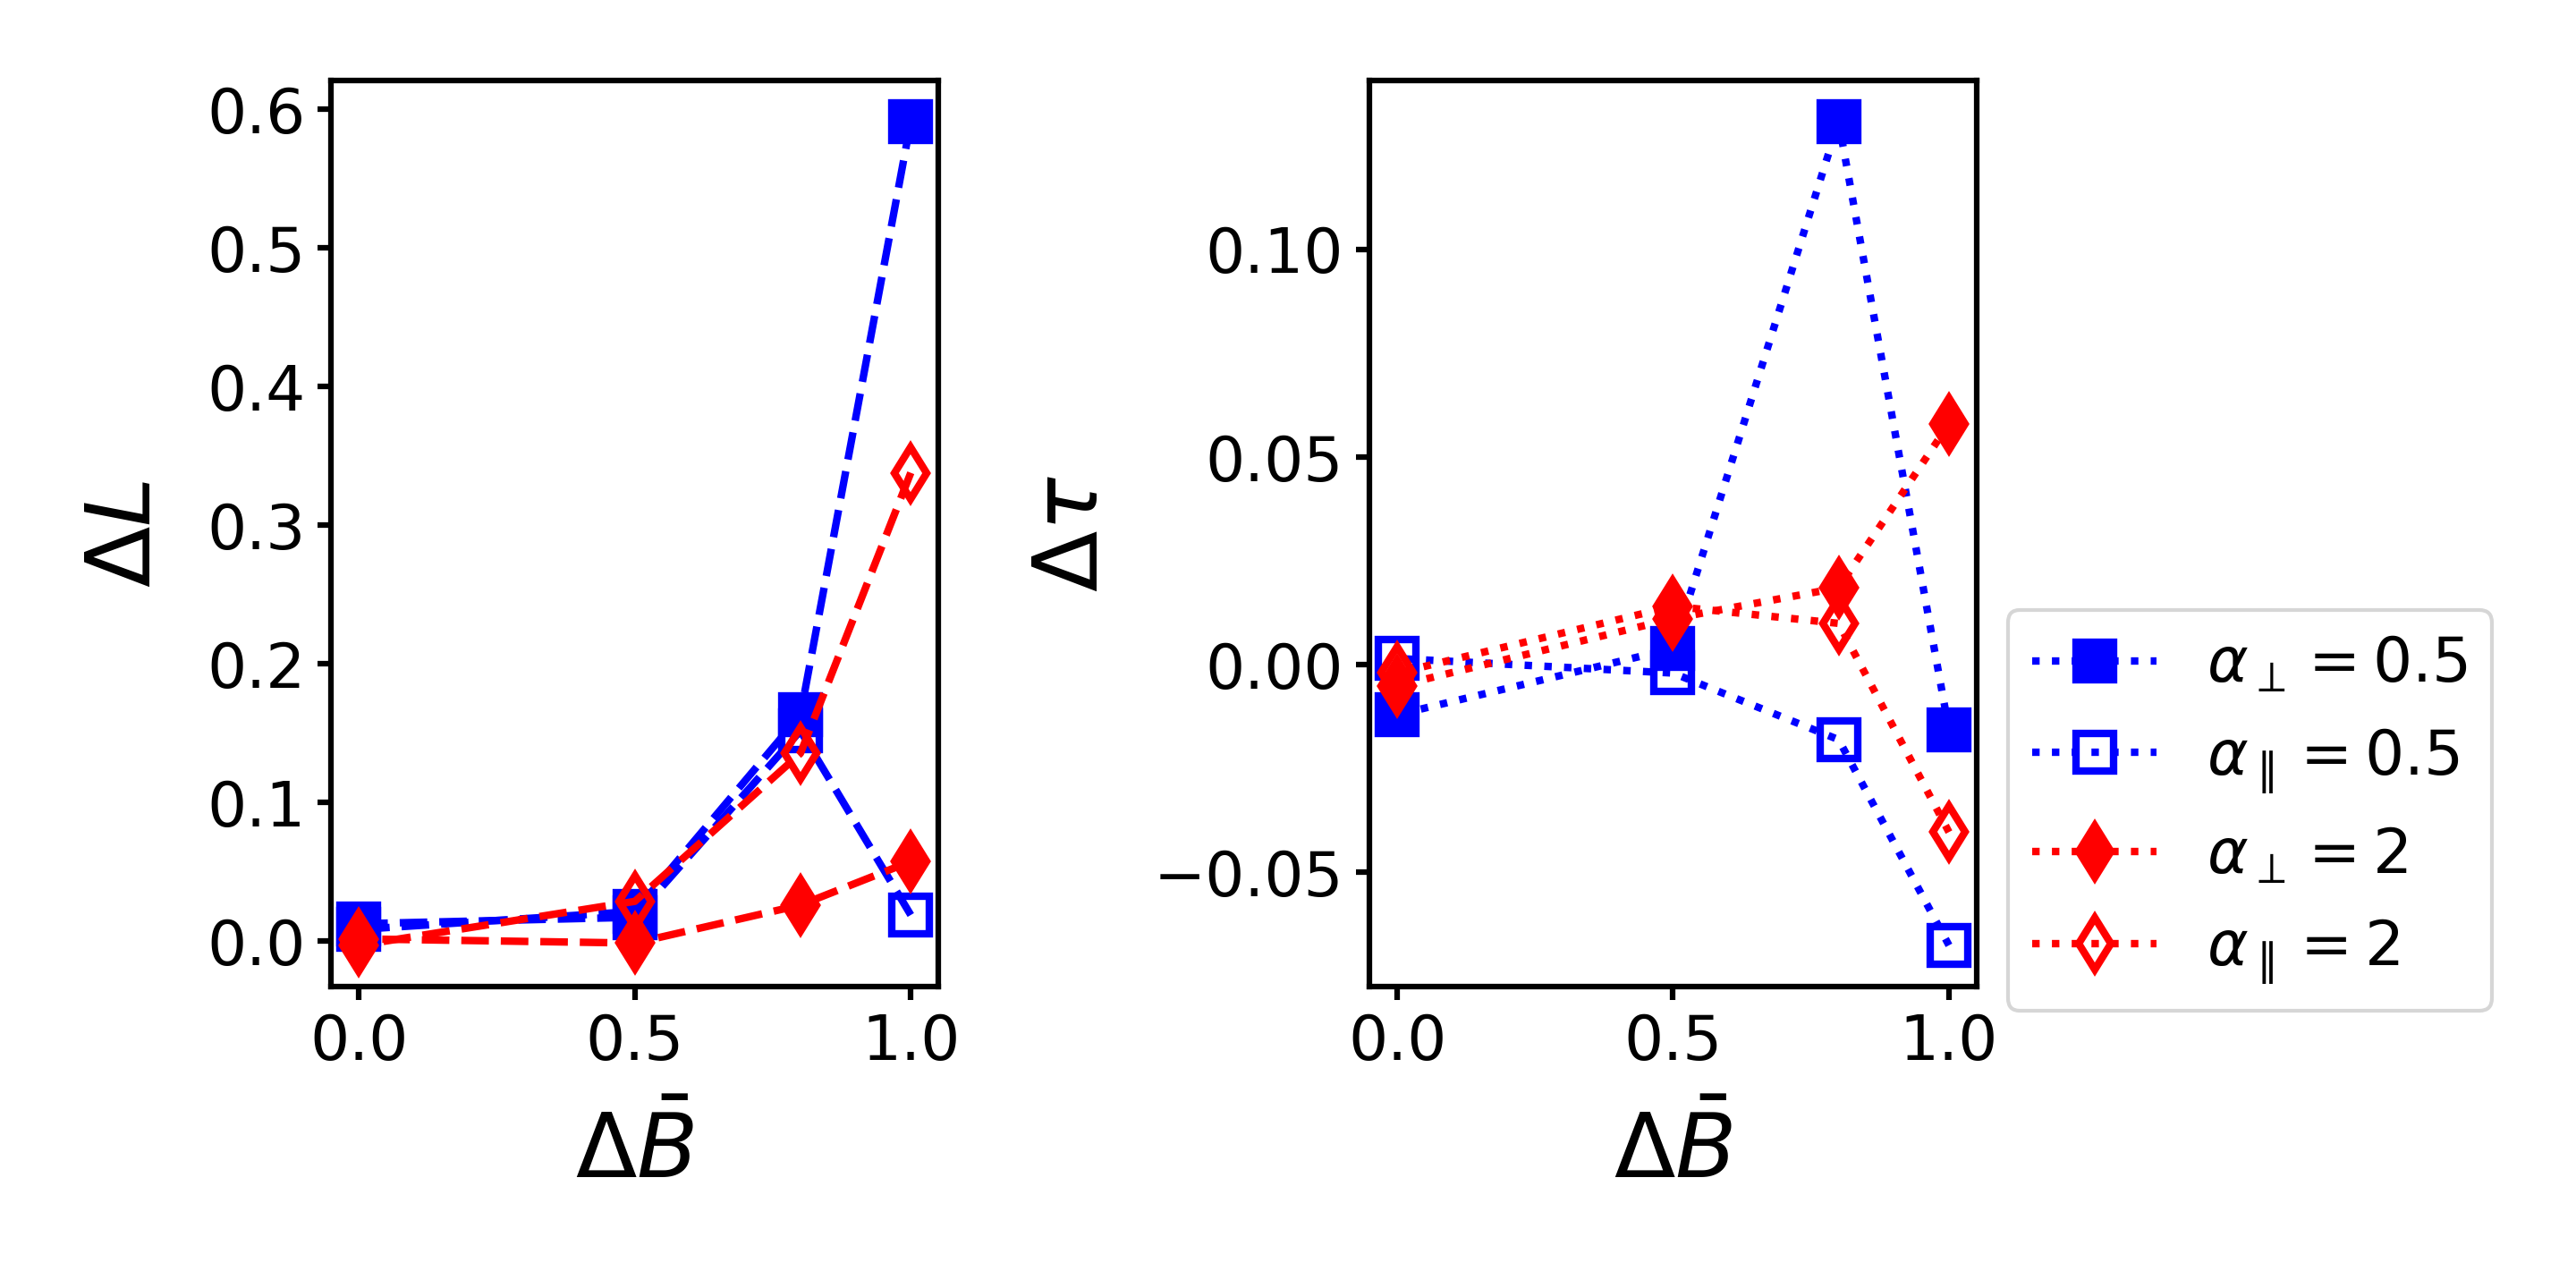
\includegraphics[scale = 0.5]{../figures/results/paper2/domain_size_aniso-field_up.png} 
\caption{Plotting the anisotropic domain sizes and tortuosity at the final timestep on the left and right respectively for bijels stabilized with oblate and prolate ellipsoidal particles starting at different particle orders. We plot these results against the change in the applied field strength, $\Delta B$. We show that the anisotropic domain size is inversely correlated to the tortuosity. We see that $L_{perp}$ changes for a bijel made with $\bar{B} = 1 \rightarrow 1$ and $\bar{B}: 0 \rightarrow 1$ differ, suggesting that the processing history of the bijel is important.} 
\label{fig:domain_size_aniso-field_up} 
\end{figure}

In Figure \ref{fig:domain_size_aniso-field_up}, we see that an increase
in the directional domain size corresponds to a decrease in the
tortuosity of the material. We also observe a magnetic field dependence
of each parameter, demonstrating that the difference in the initial and
final magnetic field applied is correlated with the domain size change
observed. Another insight is that the runs \(\bar{B}: 0 \rightarrow 1\)
and \(\bar{B}: 1 \rightarrow 1\) have different microstructural
properties. This suggests that the processing history of a bijel is
important when deciding what morphology functions ideally in a desired
application. As in above, we turn to look at the properties of the
particle monolayer. We begin by visualizing the particle monolayer in
Figure \ref{fig:particle_viz-field_up}.

From Figure \ref{fig:domain_size_aniso-field_up}, we see that domain
size anisotropy is observed upon increasing the applied field
application of the field for both particle morphologies. We also see
some domain anisotropy with no applied field, which increases upon
application of the magnetic field. The directional domain sizes,
\(L_{\perp}\) and \(L_{\parallel}\) increase by \(73\%\) and \(7\%\)
respectively for oblate particles and \(10\%\) and \(44\%\) respectively
for prolate particles. The axes that coarsens the most is consistent
with past work, explained through the directions particles reorient in
response to the applied magnetic field. In Figure
\ref{fig:domain_size_aniso-field_on}, we demonstrate that the
application of the magnetic field changes the domain size. The
tortuosity of the bijel is initially around \(\tau \approx 1.5\),
consistent with simulations of the diffusive tortuosities of gyroid
structures using Lattice Boltzmann simulations.
\cite{luo_macroscopic_2020} Upon application of the field,
\(\tau_{\perp}\) slightly decreases while \(\tau_{\parallel}\)
increases. We have seen that an increasing domain size decreases the
tortuosity in our past work. \cite{karthikeyan_formation_2024} This
observation is in line with the domain size changes observed in Figure
\ref{fig:domain_size_aniso-field_on}. The results show that the
tortuosity of the bijel is noticeably affected by the application of
magnetic fields.

As particles unjam and rejam at the interface due to reorientating to
the magnetic field, they adopt direction specific surface coverages
which manifest as anistropic domains upon jamming. The direction of the
anisotropy is different as the oblate particles have an axis of symmetry
in the short axis of the radius, while for the prolate particles it is
on the long axis. Thus during reorientation, the long axis of the oblate
particles will be orthogonal to the applied field and parallel for the
prolate particles. To characterize how the particle order changes on the
interface as a function of the magnetic field strength, we visualize the
particle monolayer of bijels stabilized by prolate particles in Figure
\ref{fig:particle_viz-field_up}.

\begin{figure} 
\centering 
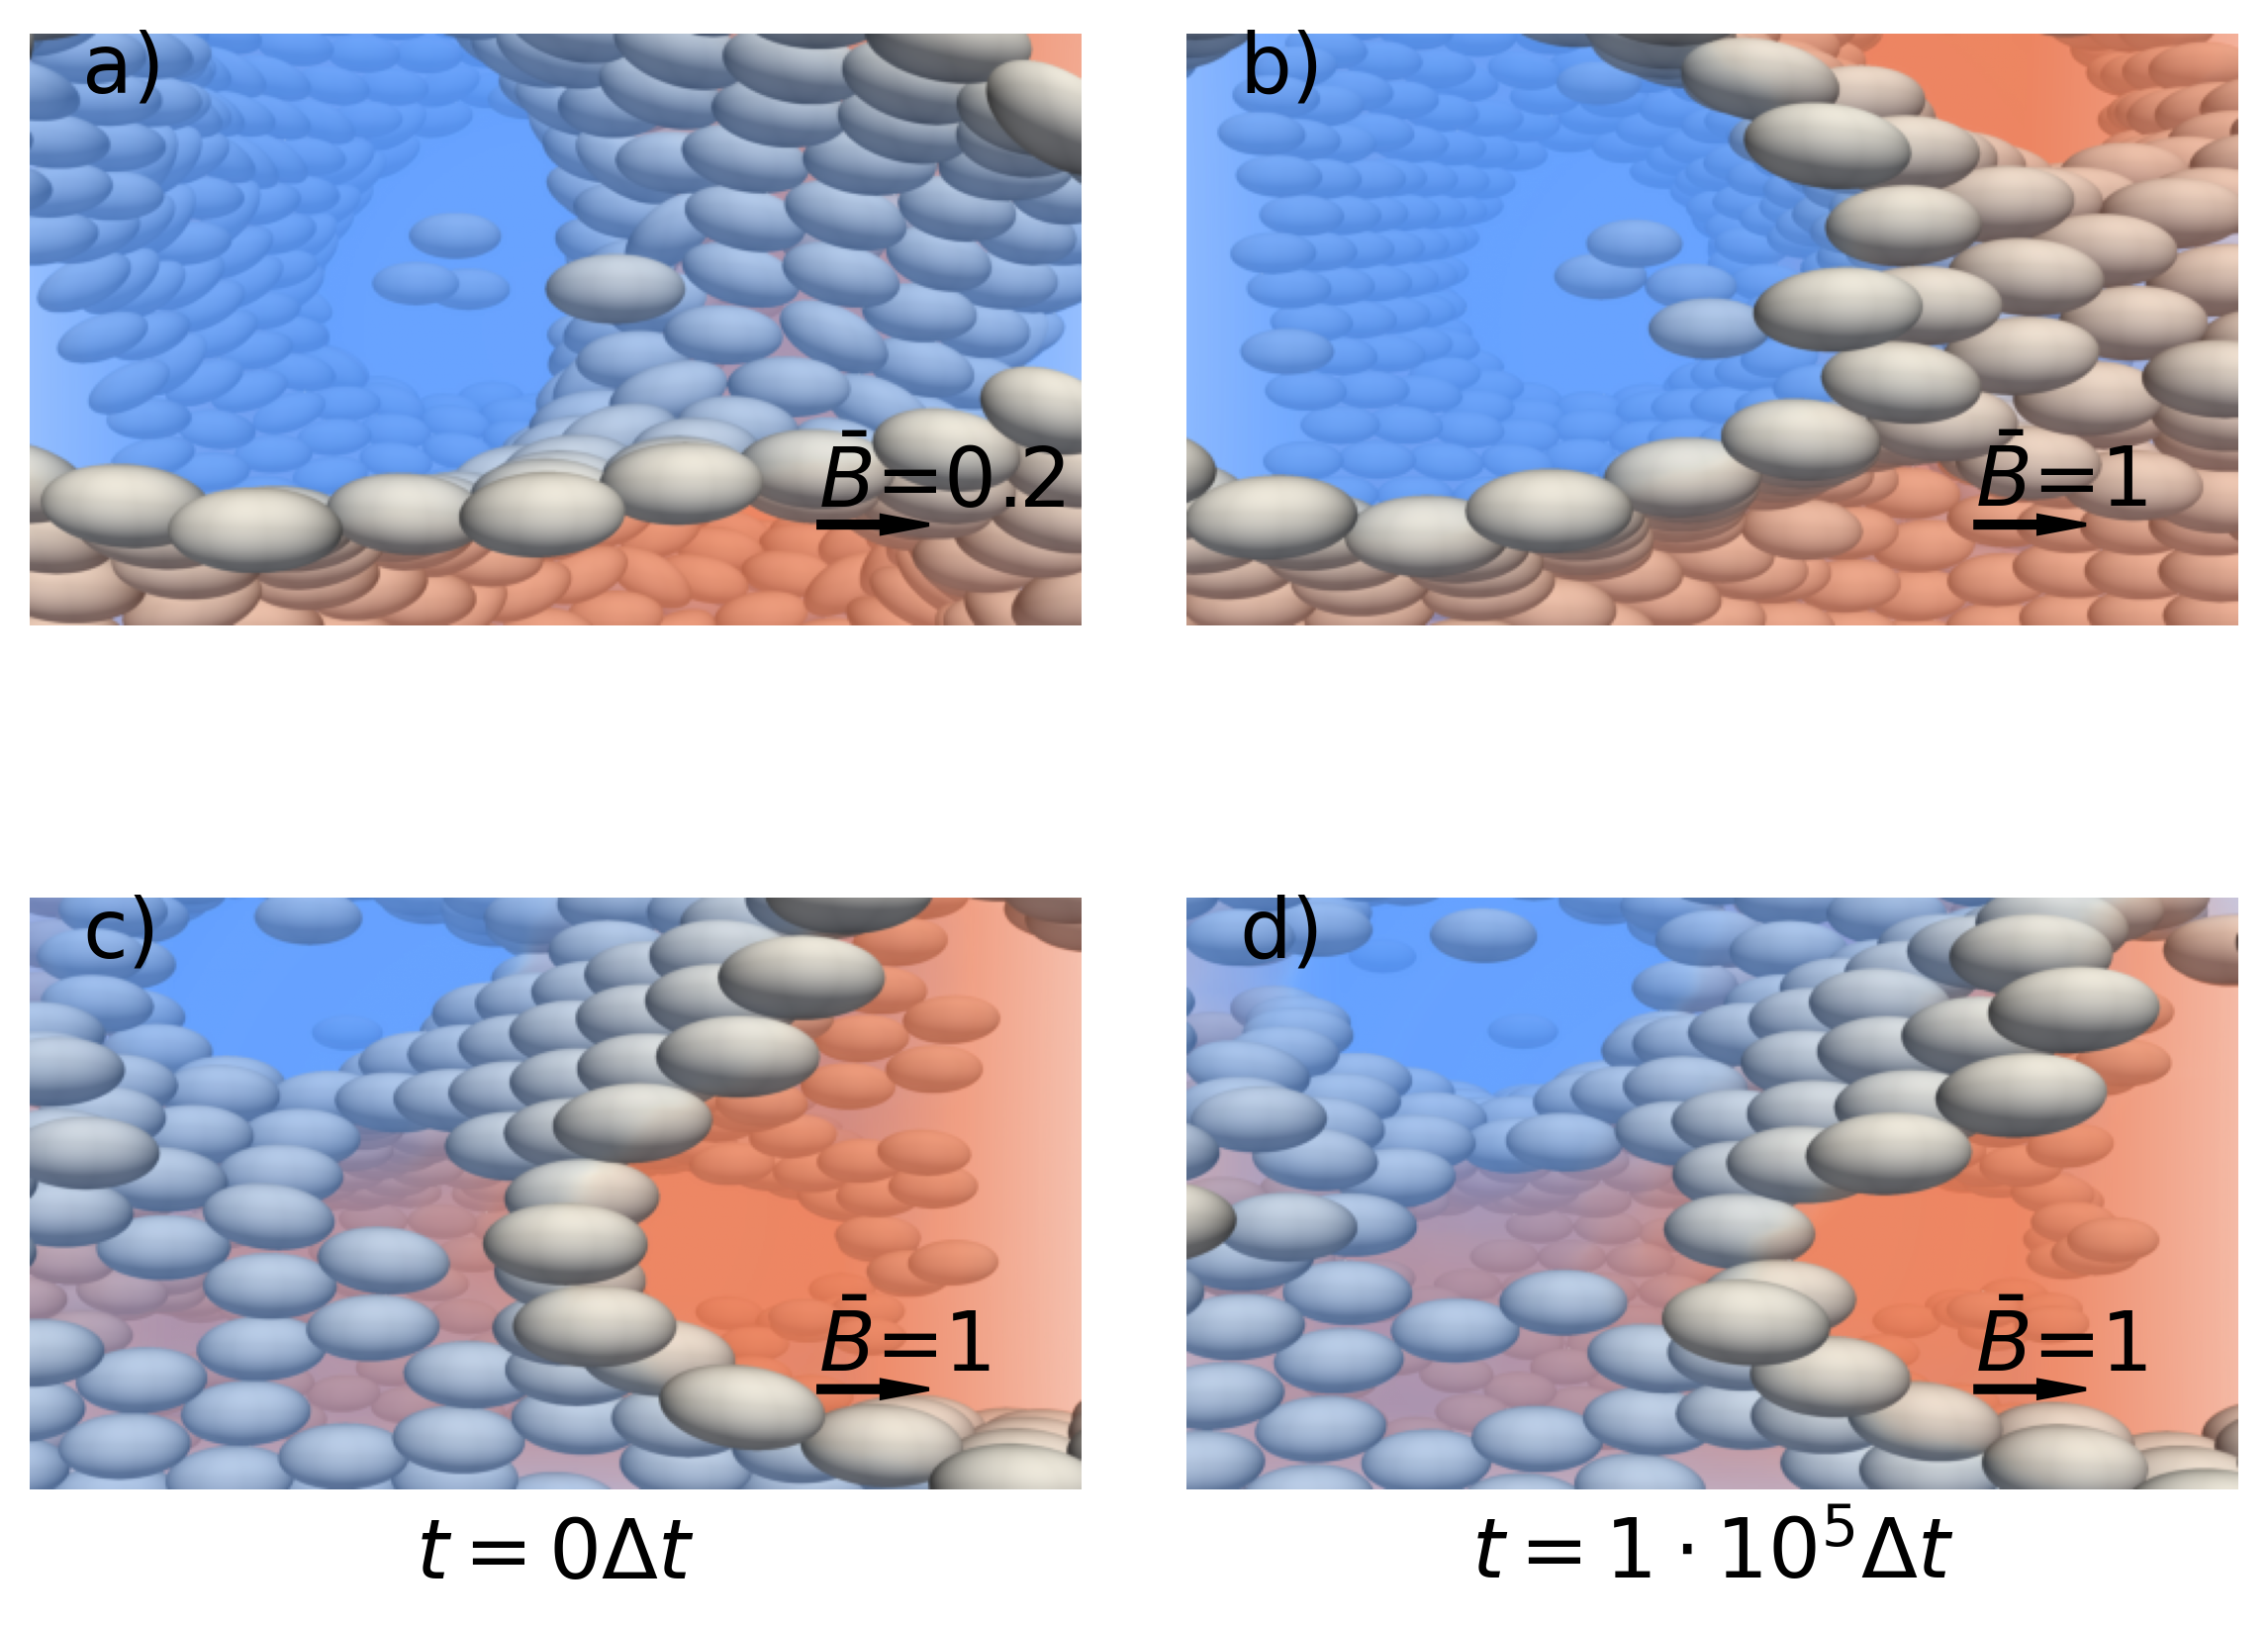
\includegraphics[scale=0.2]{../figures/results/paper2/particle_viz-field_up.png} 
\caption{Visualizations of bijels stabilized with oblate and prolate particles simulated at $t = 0$ (left column) and $t = 10^5$ (right column). The first and third rows show the particle monolayer of bijels stabilized with oblate and prolate ellipsoids respectively with an applied field of $\bar{B}_z = 0.2$. The second and fourth rows show the particle monolayer of bijels stabilized with oblate and prolate ellipsoids respectively with an applied field of $\bar{B}_z = 1$. We increase the applied field to $\bar{B}_z = 1$ in both cases and show that particle reorientation to the field occurs at the $\bar{B}_z = 0.2$ but not in the $\bar{B}_z = 1$ case.} 
\label{fig:particle_viz-field_up} 
\end{figure}

In Figure \ref{fig:particle_viz-field_up}, we see the effect of the
application of the magnetic field on the monolayer. The initial
configuration of particles at the monolayer show that even at initial
configuration of run \(\bar{B}: 0.2 \rightarrow 1\), most particles are
oriented towards the field. Upon increasing the field strength to
\(\bar{B} = 1\), all particles shown can be seen to be ordered to the
field, matching the results for the nematic order parameter shown in
Figure \ref{fig:domain_size-field_up}. We also observe the alignment of
the long axis of the particles to the magnetic field, demonstrating the
origin of the microstructure anisotropy. To understand how the particle
reorientation at the interface causes microstructure reorientation we
quantify the average interface angle, \(\langle \psi \rangle\) and the
local interface order of the material, \(\langle Q_6 \rangle\) in Figure
\ref{fig:interface_angle-nint-field_up}.

\begin{figure} 
\centering 
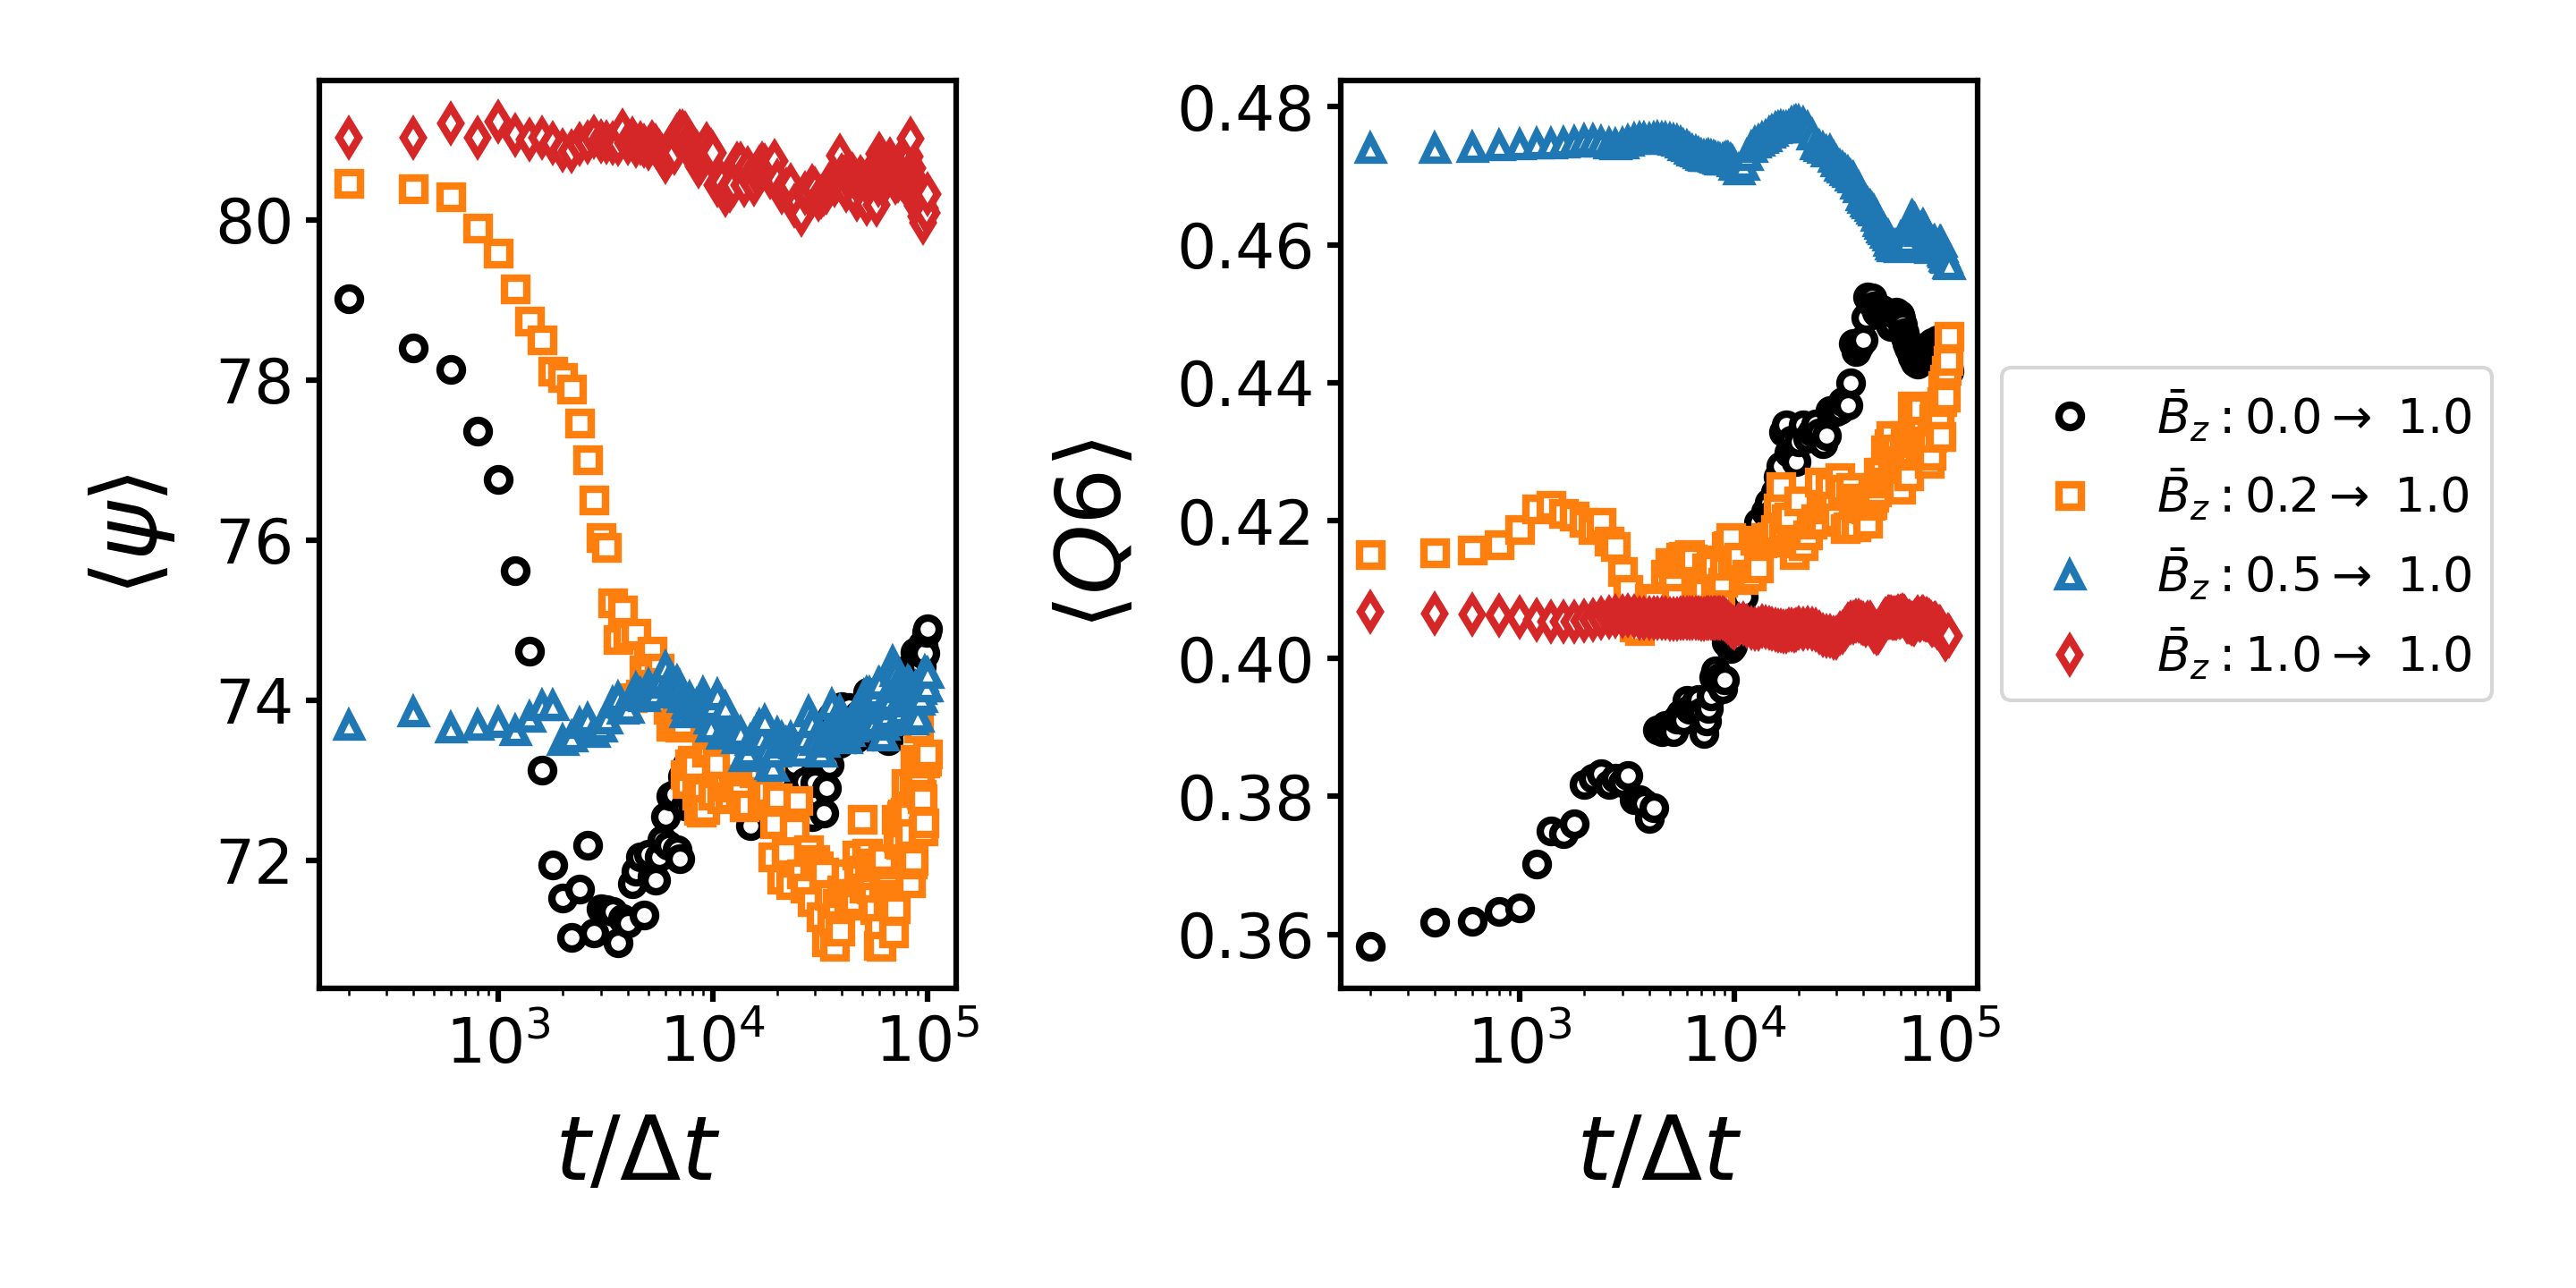
\includegraphics[scale=0.4]{../figures/results/paper2/interface_angle-nint-field_up.png} 
\caption{Plots of the average interfacial angle $\psi$ and the number of particles on the interface $n_{int}$ on the left and right respectively, plotted against time for bijels stabilized with ellipsoidal particles with aspect ratio 2. When looking at $\psi$, a change in dynamics can be seen as the initial particle order increases. When looking at $n_{int}$, different dynamics are seen above and below the isotropic to nematic transition point. Both results suggest that the ordering of particles is linked to the dynamics of domain coarsening.} 
\label{fig:interface_angle-nint-field_up} 
\end{figure}

From Figure \ref{fig:interface_angle-nint-field_up}, we identify that
prolate and oblate particles respond differently at the interface. We
show that there are three time evolution trends for
\(\langle \psi \rangle\) and \(\langle Q_6 \rangle\) for both oblate and
prolate particles despite the differences in the initial state of the
particles. In oblate particles \(\langle \psi \rangle\) begins closer to
\(0 ^{\circ}\) as the axis of symmetry lies close to the interface
normal. We see that for bijels experiencing a field strength history of
\(\bar{B}: 0 \rightarrow 1\) and \(\bar{B}: 0.2 \rightarrow 1\),
\(\langle \psi \rangle\) increases, plateaus and increases again before
plateauing again. This is indicative of particles tilting at the
interface, before interfacial capillary interactions ``pause'' particle
reorientation before the applied magnetic field begins to cause
particles to tilt out of the interface. We see similar trends for bijels
stabilized by prolate particles. \(\langle \psi \rangle\) begins near
\(80 ^{\circ}\). We see a decrease before reorientation ceases, and
finally \(\langle \psi \rangle\) increases again.

When looking at \(\langle Q_6 \rangle\) for \(\bar{B}: 0 \rightarrow 1\)
and \(\bar{B}: 0.2 \rightarrow 1\) for oblate particles, we see that the
trends are similar with an initial decrease, followed by a plateau and
increase over time before plateauing again. \(\langle Q_6 \rangle\)
generally decreases with a large decrease observed for
\(\bar{B}: 0 \rightarrow 1\) from an initial hexagonally packed system
to a structure that is locally ordered but not close packed. For prolate
particles, we see an increase in \(\langle Q_6 \rangle\) with a plateau
occurring in both systems around 5000 timesteps. The significance of
this time is unknown for \(\bar{B}: 0.2 \rightarrow 1\) but for
\(\bar{B}: 1 \rightarrow 1\), this is approximately the local
crystallization point when \(\langle Q_6 \rangle \geq 0.38\).

For oblate particles, we can conclude that structural response dynamics
arise from particle tilting on the interface identified as the large
difference between the initial and final \(\langle \psi \rangle\) with
an associated decrease in the interface coverage, initiating domain
coarsening. We see that this interfacial tilting causes a loss in the
close packing of oblate particles at the interface. For prolate
particles, we observe a small degree of particle tilting as can be seen
from \(\langle \psi \rangle\), although the dynamics are primarily
driven by the change in \(\langle Q_6 \rangle\), indicated as a slight
dip and plateau before the particles begin reordering and packing more
tightly, decreasing the interfacial area. Larger domain size response is
observed for the prolate particles as the interfacial area change from
particle tilting at the interface is larger than that of particles close
packing at the interface.

For both particle morphologies we analyze the response of bijels with a
field history of \(\bar{B}: 0.5 \rightarrow 1\) and
\(\bar{B}: 1 \rightarrow 1\). We see a decrease in
\(\langle Q_6 \rangle\) for bijels stabilized with oblate particles with
field application of \(\bar{B}: 0.5 \rightarrow 1\) compared to an
increase for \(\bar{B}: 1 \rightarrow 1\). This behavior arises from the
slight increase in the nematic order for particles in bijels
experiencing the \(\bar{B}: 0.5 \rightarrow 1\) field application
history. The \(\langle \psi \rangle\) results indicate that the
particles rearrange over time to lie flatter on the interface. For
bijels stabilized with prolate particles, we characterize a difference
in behavior between \(\bar{B}: 0.5 \rightarrow 1\) and
\(\bar{B}: 1 \rightarrow 1\). For the \(\bar{B}: 0.5 \rightarrow 1\)
case, we see a slight increase in \(\langle \psi \rangle\) before a
decrease and increase compared to the \(\bar{B}: 1 \rightarrow 1\) case
where we characterize a slight decrease over time. We also characterize
a slight decrease in \(\langle Q_6 \rangle\) over time for the
\(\bar{B}: 1 \rightarrow 1\) case while characterizing a larger decrease
for the \(\bar{B}: 0.5 \rightarrow 1\) case. Similar to the oblate
particles, these results originate from the slight increase in the
nematic order for bijels experiencing the \(\bar{B}: 0.5 \rightarrow 1\)
field history.





\subsection{Decreasing the applied
field}\label{decreasing-the-applied-field}

Bijels are kinetically stable structures whose properties are dependent
upon the stability of the particle monolayer. Past work into responsive
emulsions have demonstrated resilience to microstructure changes after
application and removal of stimuli even after several months. However,
in the systems simulated above the particles need not necessarily be in
thermodynamically stable states when jammed upon removal of stimuli as
the particles take up a arrangements not observed when no field is
applied. In this section, we explore how removal of the magnetic field
changes the microstructure of the bijel as a function of the initial
particle order. We use bijels simulated under
\(\bar{B}_{template} = 0, 0.2, 0.5, 1\) during phase separation. Once
the microstructure has stabilized, we switch off the magnetic field and
observe the time evolution of the system for \(t = 10^5\) timesteps.

\begin{figure} 
\centering 
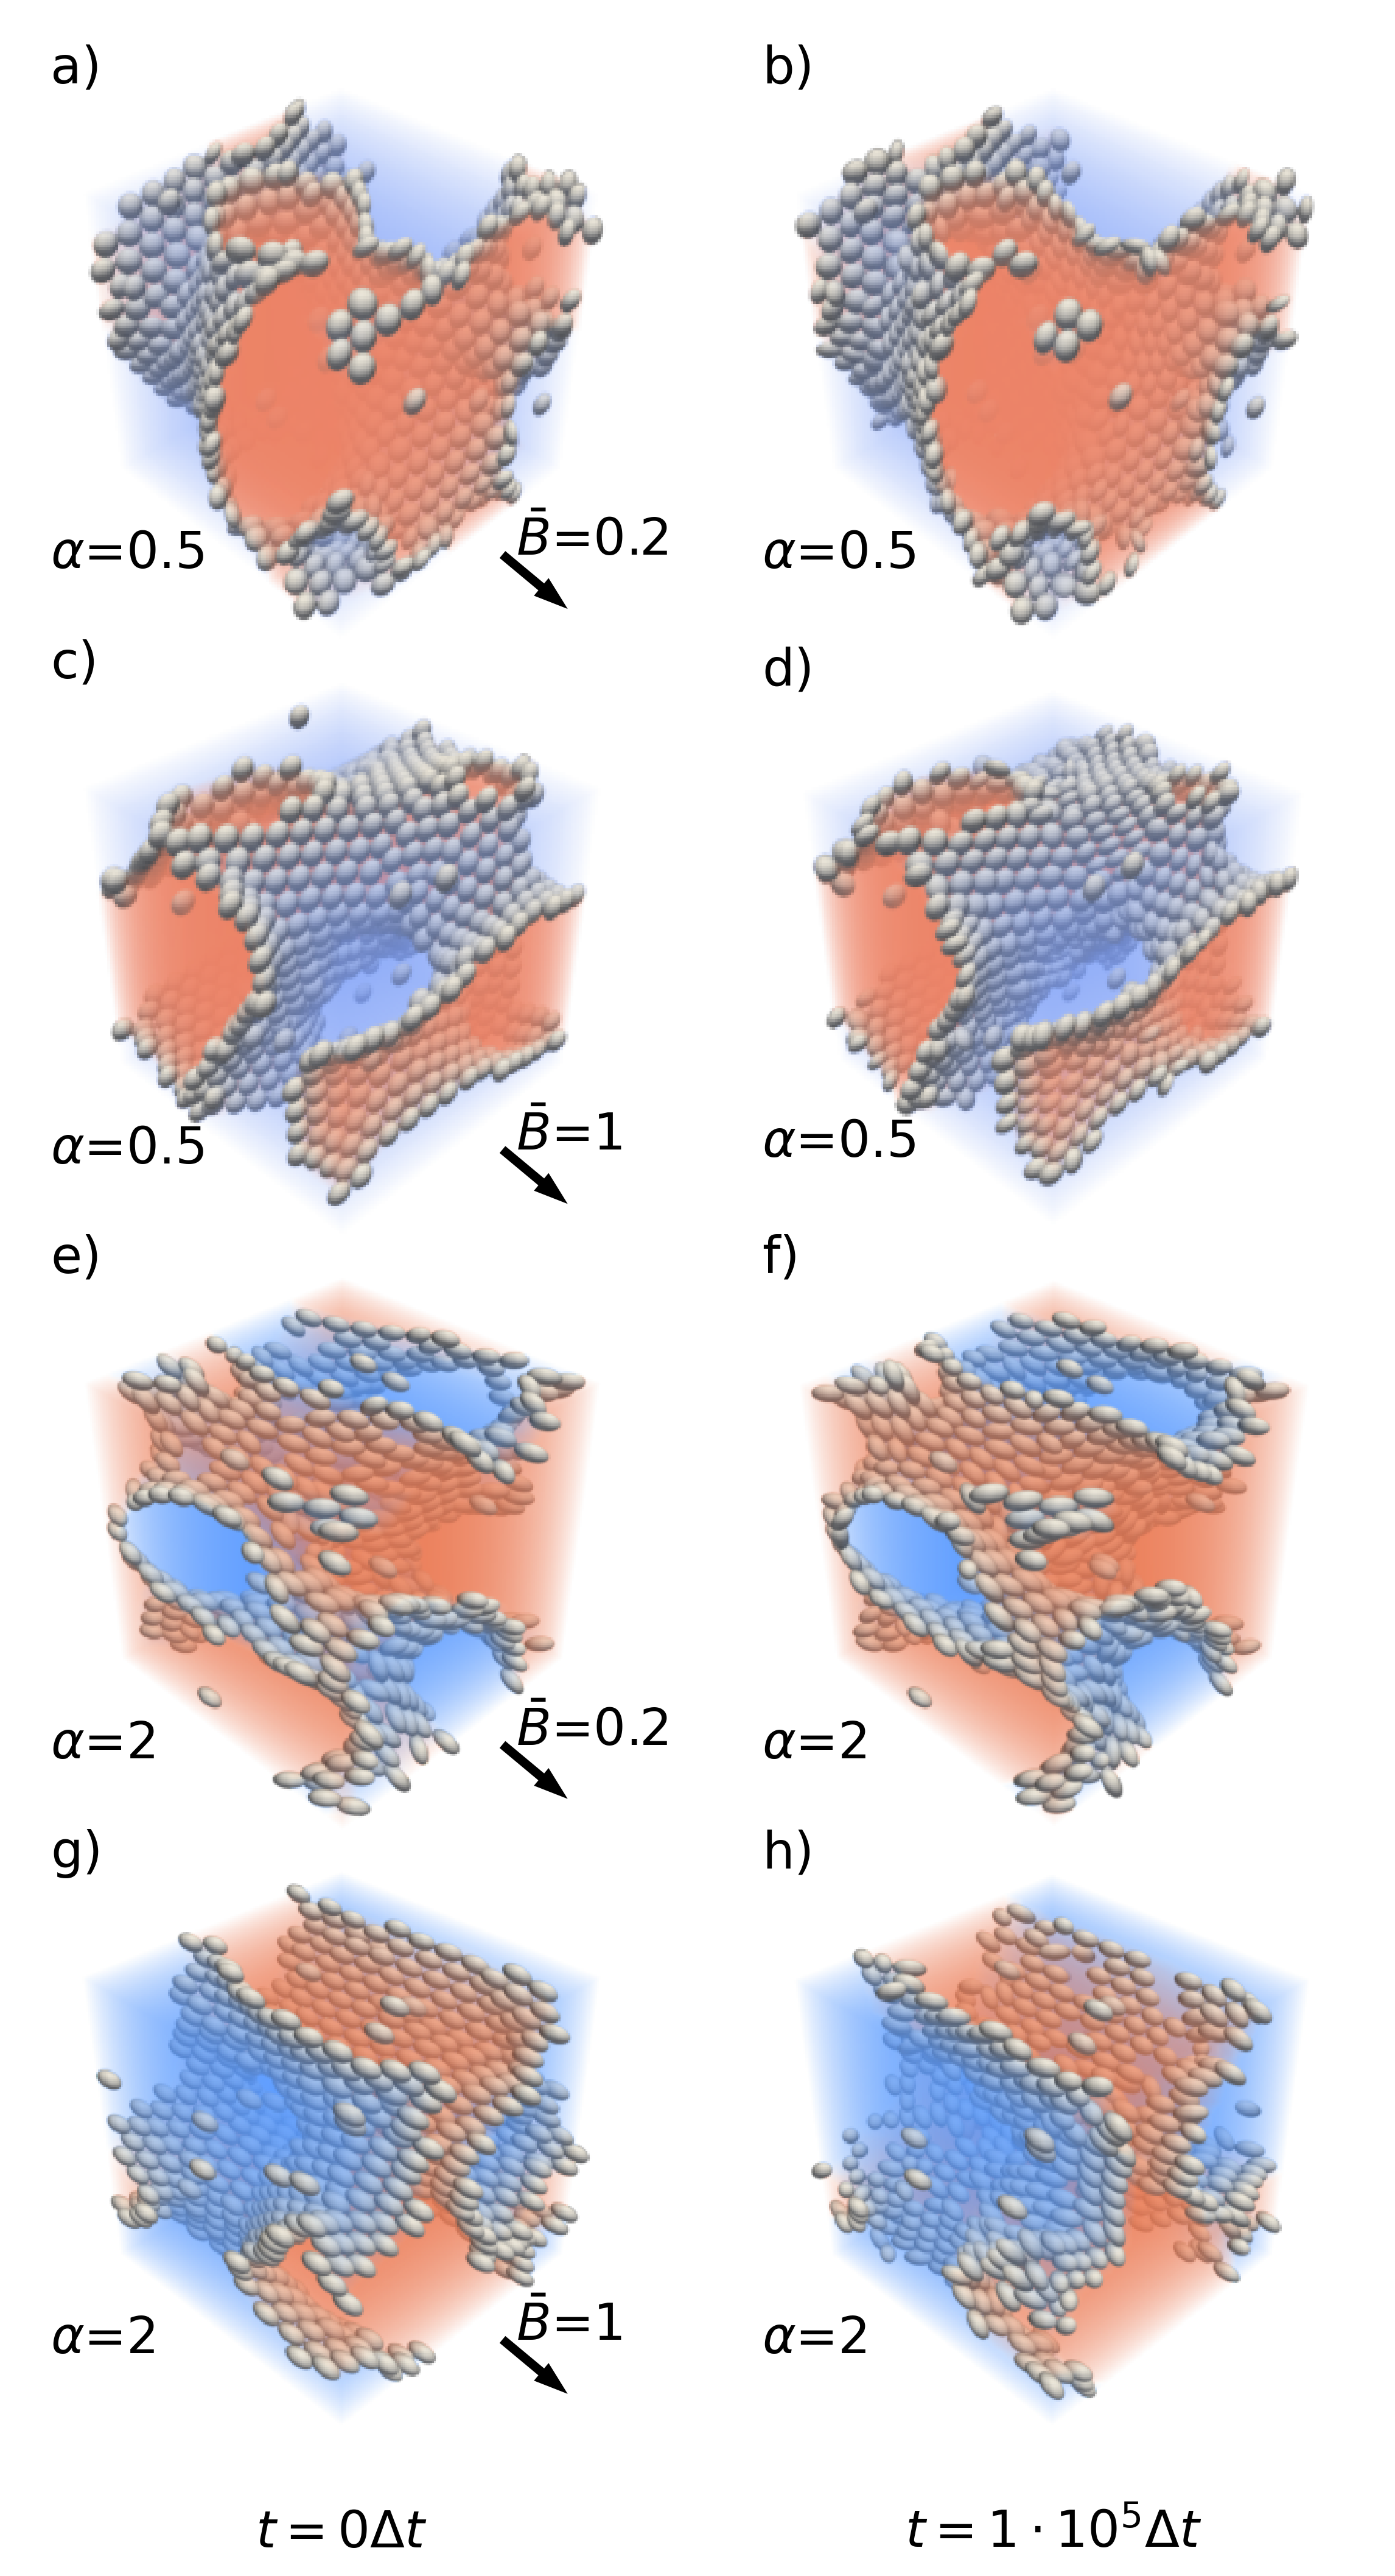
\includegraphics[scale=0.4]{../figures/results/paper2/microstructure_viz-field_down.png} 
\caption{Visualizations of bijels stabilized with oblate and prolate particles simulated at $t = 0$ (left column) and $t = 10^5$ (right column). The first and third rows show the particle monolayer of bijels stabilized with oblate and prolate ellipsoids respectively with an applied field of $\bar{B}_z = 0.2$. The second and fourth rows show the particle monolayer of bijels stabilized with oblate and prolate ellipsoids respectively with an applied field of $\bar{B}_z = 1$. We switch off the applied field in both cases and show that while particle reorientation occurs, it has little effect on the microstructure of the bijel.}
\label{fig:microstructure_viz-field_down}
\end{figure}

In Figure \ref{fig:microstructure_viz-field_down}, we visualize the time
evolution of the microstructure of bijels with processing history
\(\bar{B}:0.2 \rightarrow 0\) (top) and \(\bar{B}:1 \rightarrow 0\)
(bottom). We see that when switching the field off, the microstructure
remains largely the same, demonstrating the kinetic stability of bijels.
However, the particle monolayer, while still showing order, appears to
be slowly losing that order as particles are beginning to become
randomly oriented. This is especially obvious in the
\(\bar{B}:1 \rightarrow 0\) process, demonstrating that the dynamics of
the system is dependent upon the initial order of the particle
monolayer.

\begin{figure} 
\centering 
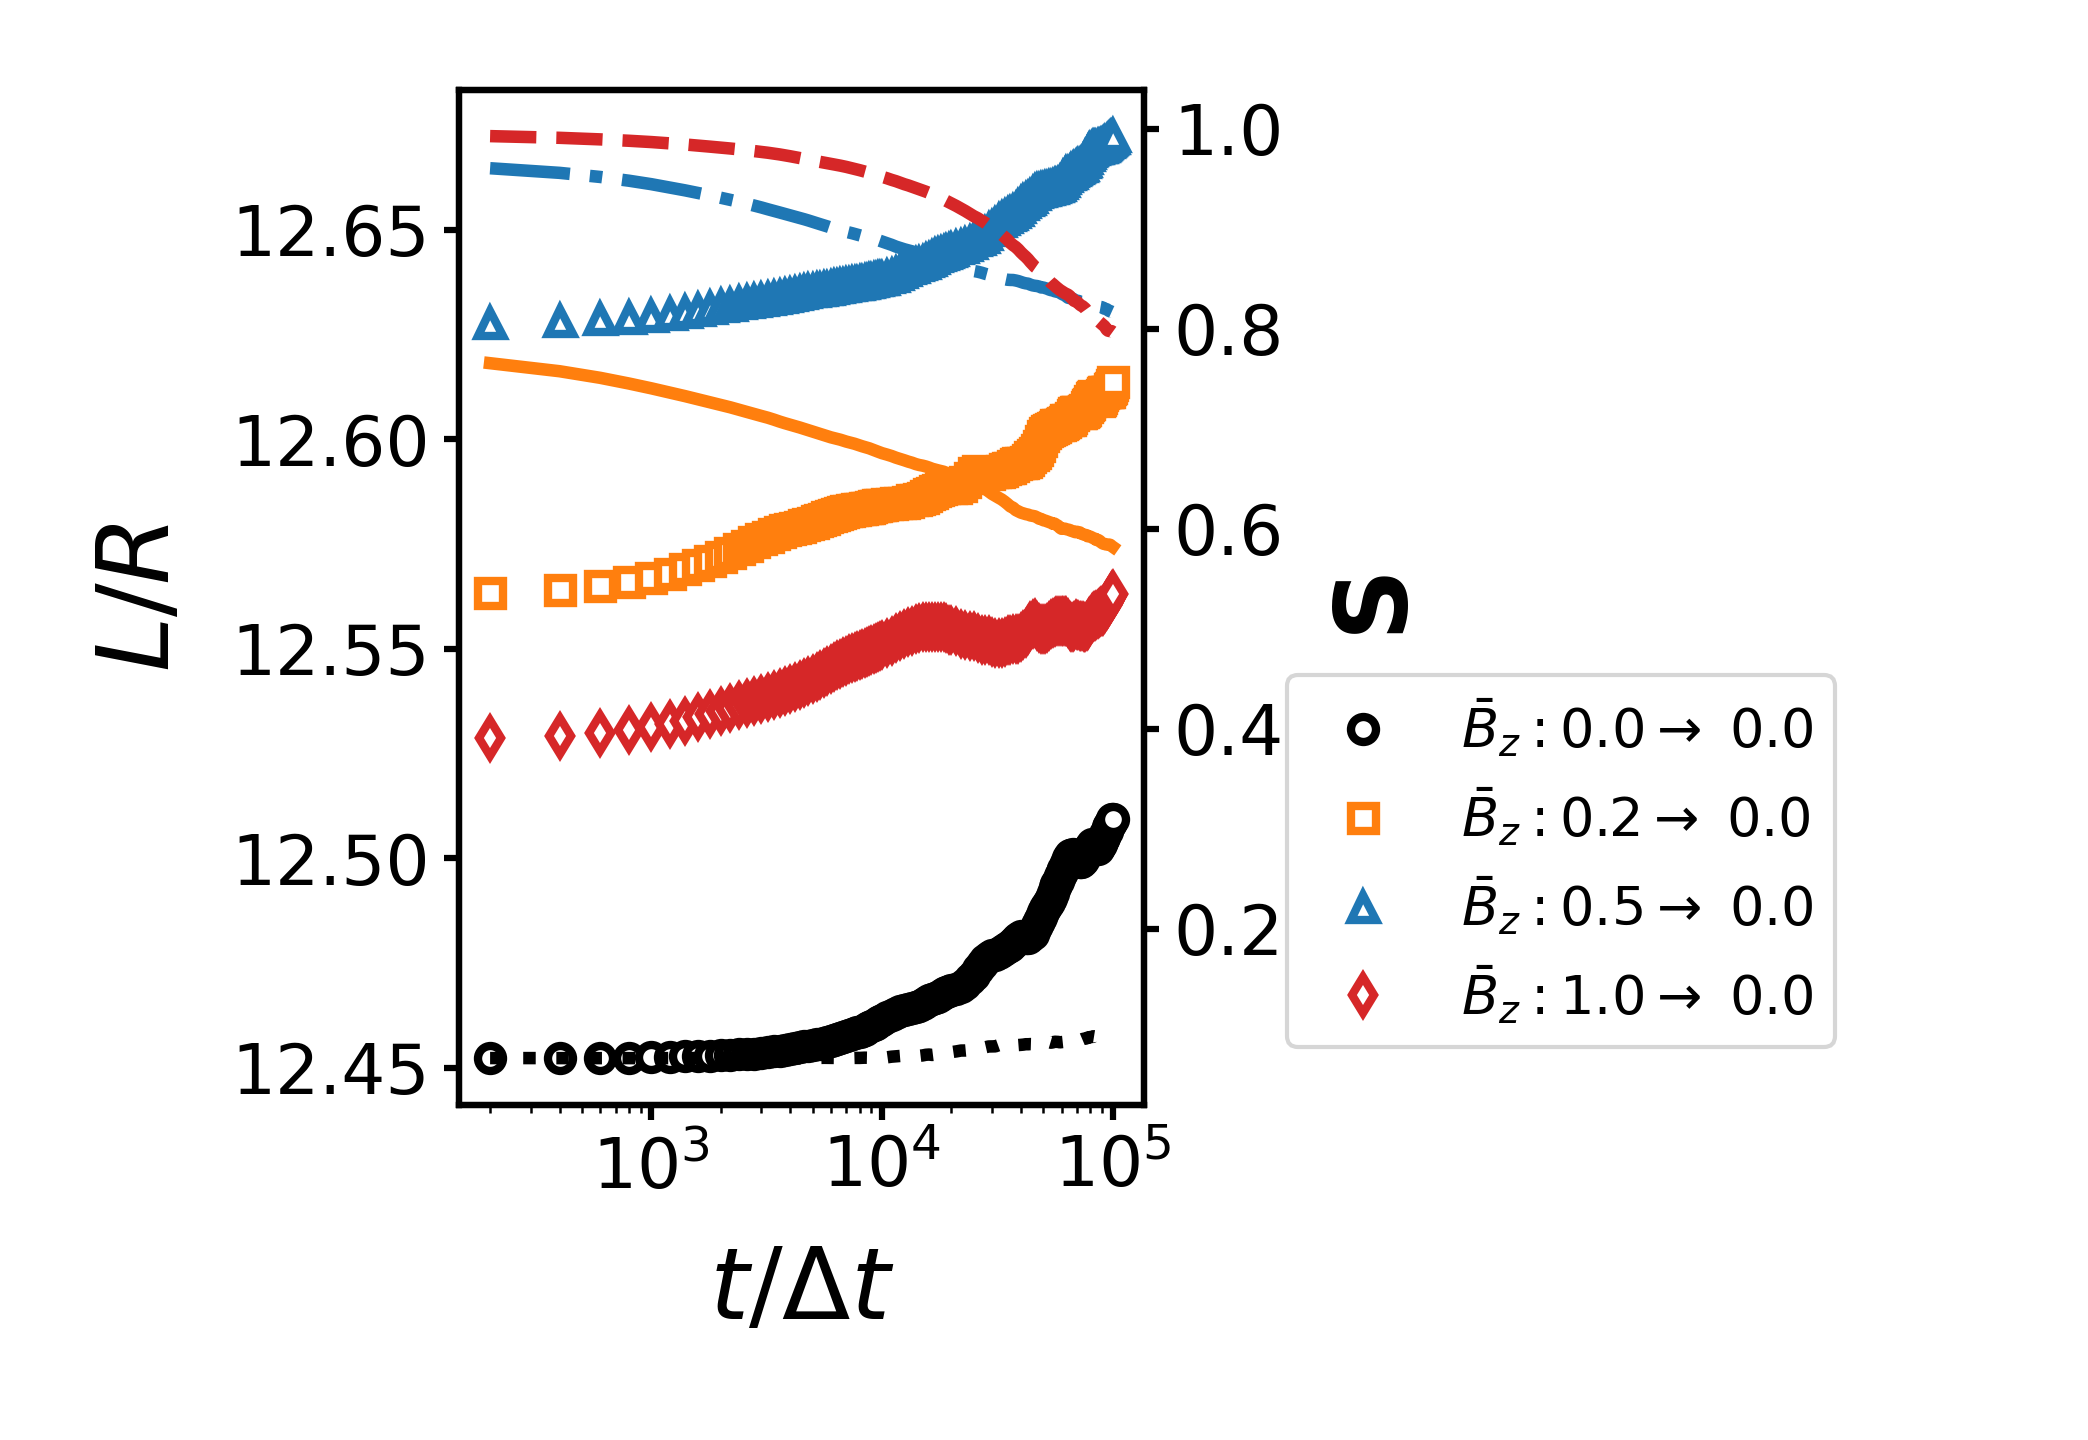
\includegraphics[scale=0.5]{../figures/results/paper2/domain_size-field_down.png} 
\caption{Plot of the spherically averaged domain size normalized with $R_p$ of the particle and the nematic order parameter of each bijel over time. Each color represents bijel templates made with different field strengths $\bar{B}$. We show that there is domain coarsening when the field is switched off, along with a reduction in the ordering of the particles.} 
\label{fig:domain_size-field_down} 
\end{figure}

From the results in \ref{fig:domain_size-field_down}, we can see that
the results show, with the exception of \(\bar{B}: 0\rightarrow 0\), all
domain sizes show a slow coarsening over time. This is reflected clearly
in the bijels stabilized by prolate particles, showing that that the
changes in properties of the particle monolayer due to the applied
magnetic field during bijel template simulation does not play a
significant role in the dynamics of the bijel. We attribute the large
increase in the domain size in oblate particle stabilized
\(\bar{B}: 0\rightarrow 0\) case to be due to coalescence of two
domains, characterized as a two step process where we see slower long
timescale domain coarsening initially followed by a rapid jump in the
domain size.

The nematic order parameter of all runs with prexisting particle order
show order dependent decreases, arising from interfacial forces causing
the particles to return to a thermodynamically optimum configuration on
the interface. To quantify is the coarsening that takes place is
anisotropic, we define the relative change in domain size as
\(\Delta L = \frac{L_{f} - L_{i}}{L_{i}}\), where \(L\) represents
either \(L_{\perp}\) or \(L_{\parallel}\). The same formulation is
applied to the tortuosity in the respective directional components. We
do this to characterize the \(\Delta \bar{B}\)-dependent changes
observed in the domain anisotropy. The results are presented in Figure
\ref{fig:domain_size_aniso-field_up}.

\begin{figure} 
\centering 
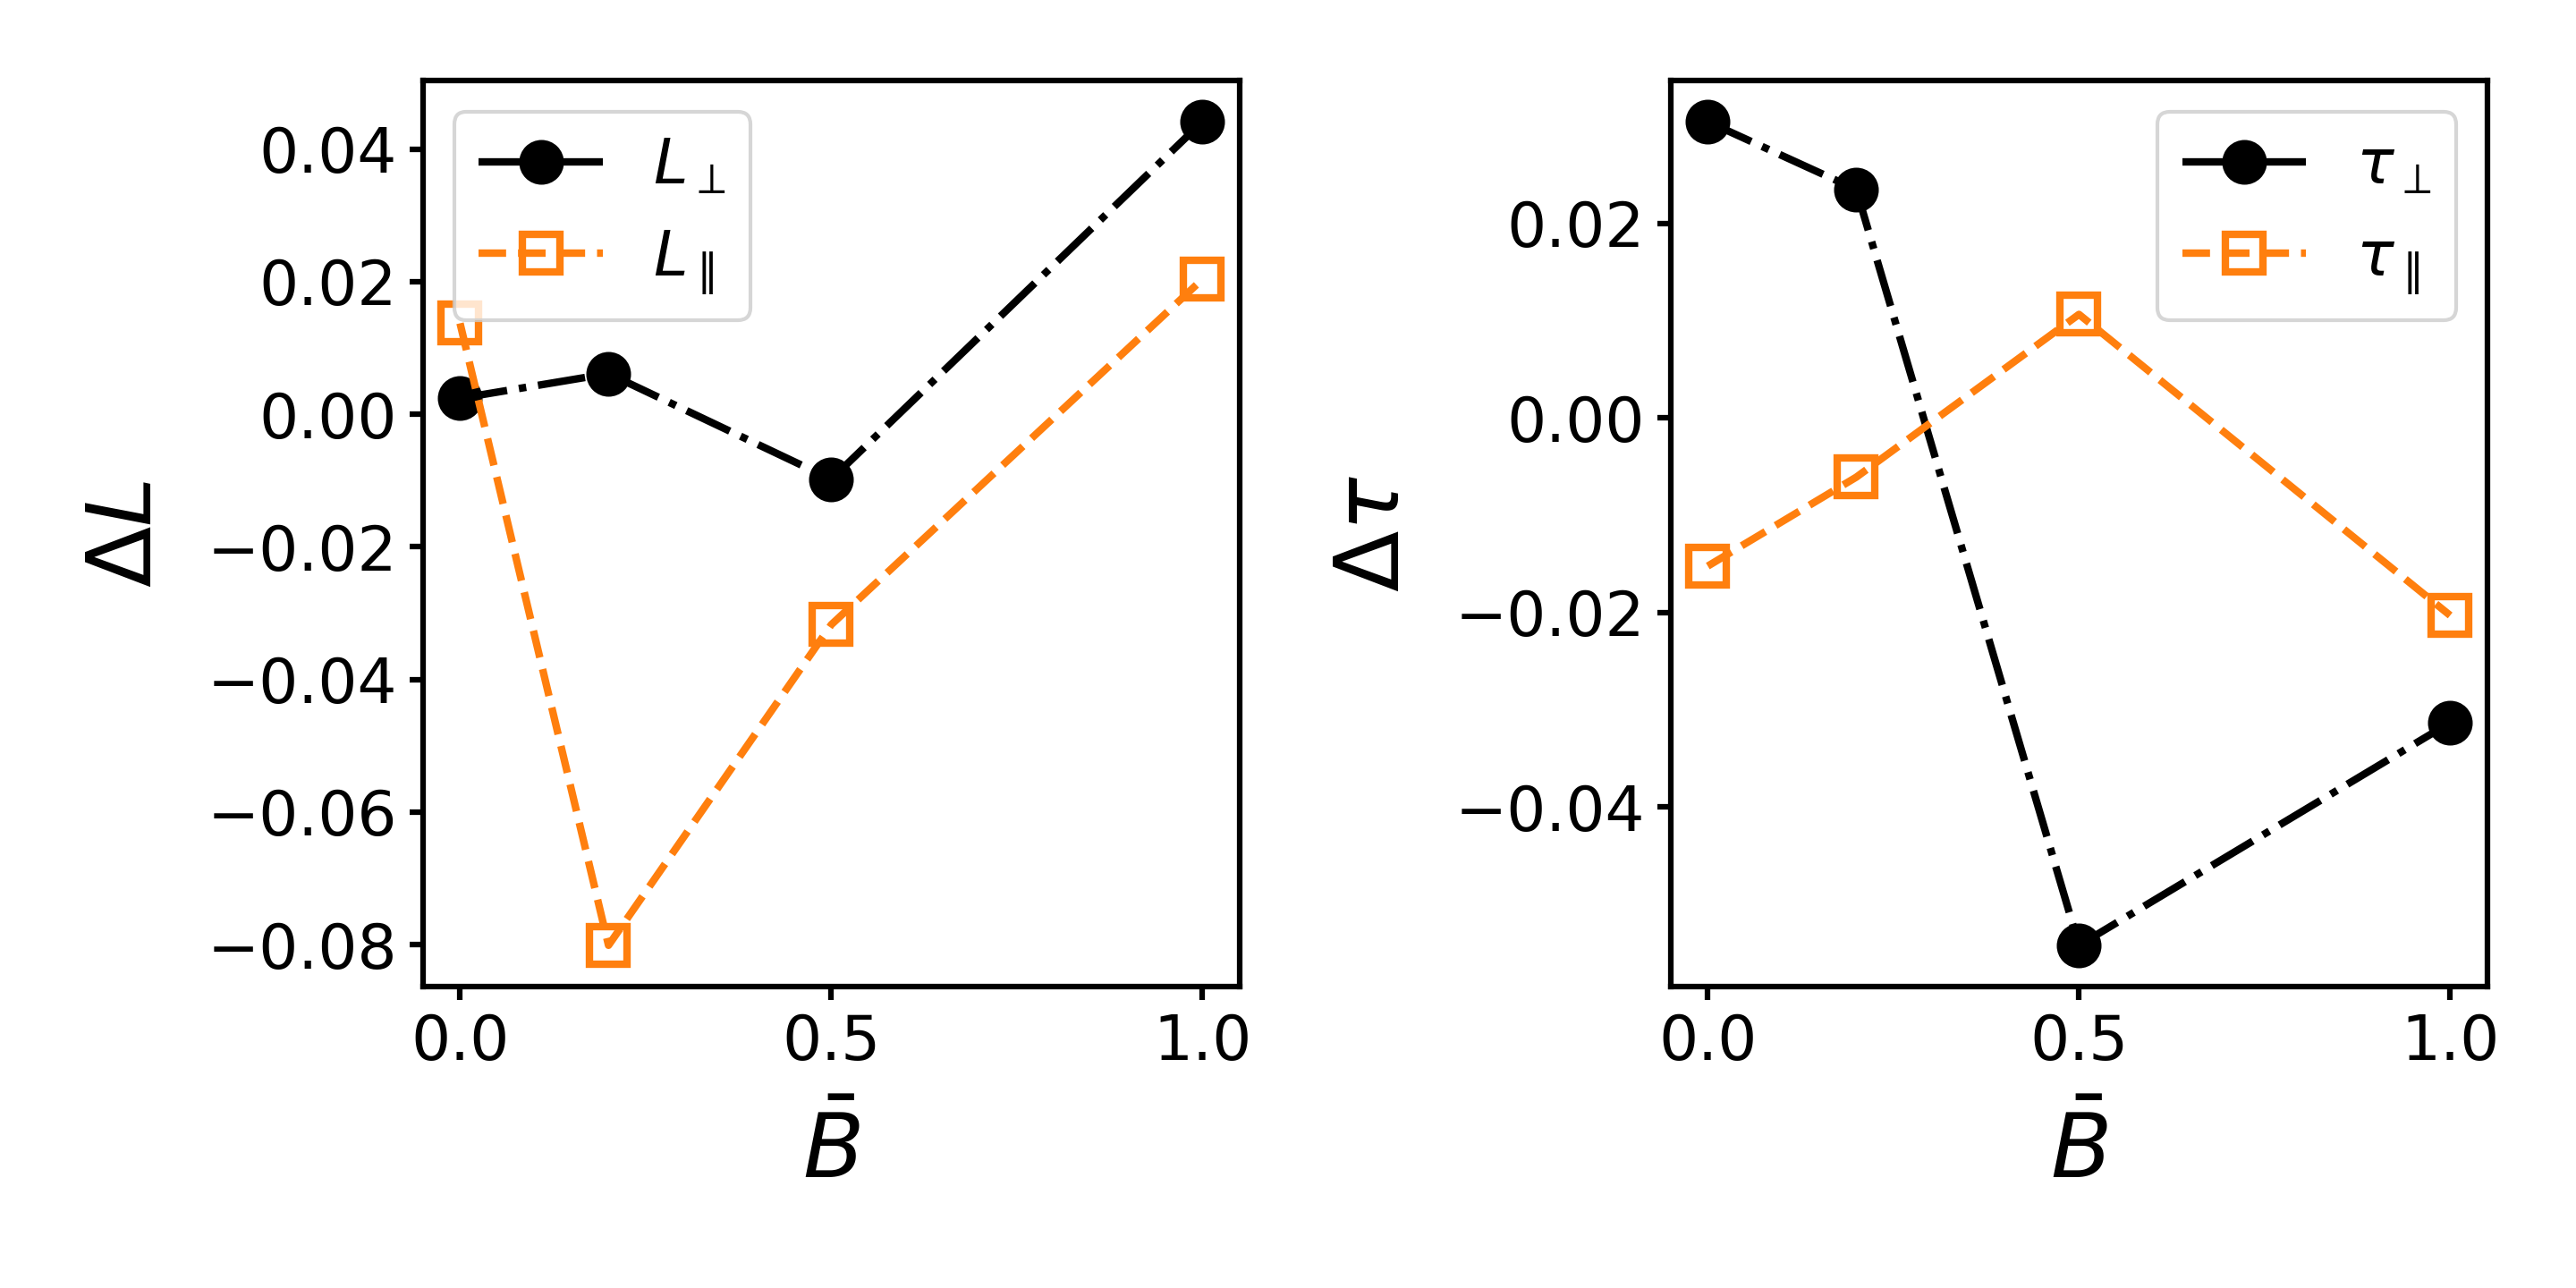
\includegraphics[scale = 0.5]{../figures/results/paper2/domain_size_aniso-field_down.png} 
\caption{Plotting the anisotropic domain sizes and tortuosity at the final timestep on the left and right respectively for bijels stabilized with oblate and prolate ellipsoidal particles starting at different particle orders. We plot these results against the change in the applied field strength, $\Delta B$. We show that there are only minor differences in the microstructure of stimuli responsive bijels once the magnetic field is switched off.} 
\label{fig:domain_size_aniso-field_down} 
\end{figure}

In Figure \ref{fig:domain_size_aniso-field_down}, we see that there are
small \(\Delta \bar{B}\) dependent changes in the anisotropic domain
size and tortuosity for both particle morphologies. However, there are
no clear trends that can be developed from these plots, suggesting that
the changes are overall isotropic and any differences observed arise
from the arrangement of particles. This suggests that the response of
the material to the removal of a magnetic field is isotropic and only
dependent upon the capillary interactions with the particle monolayer.
We showed earlier that the application of magnetic fields change the
local state of the particles at the interface. However the results shown
thus far demonstrate that that these changes do not seem to affect the
coarsening of the bijel once stimuli is removed. To investigate why this
is the case, we plot \(\langle \psi \rangle\) and
\(\langle Q_6 \rangle\) for bijels stabilized with ellipsoidal particles
below.

\begin{figure} 
\centering 
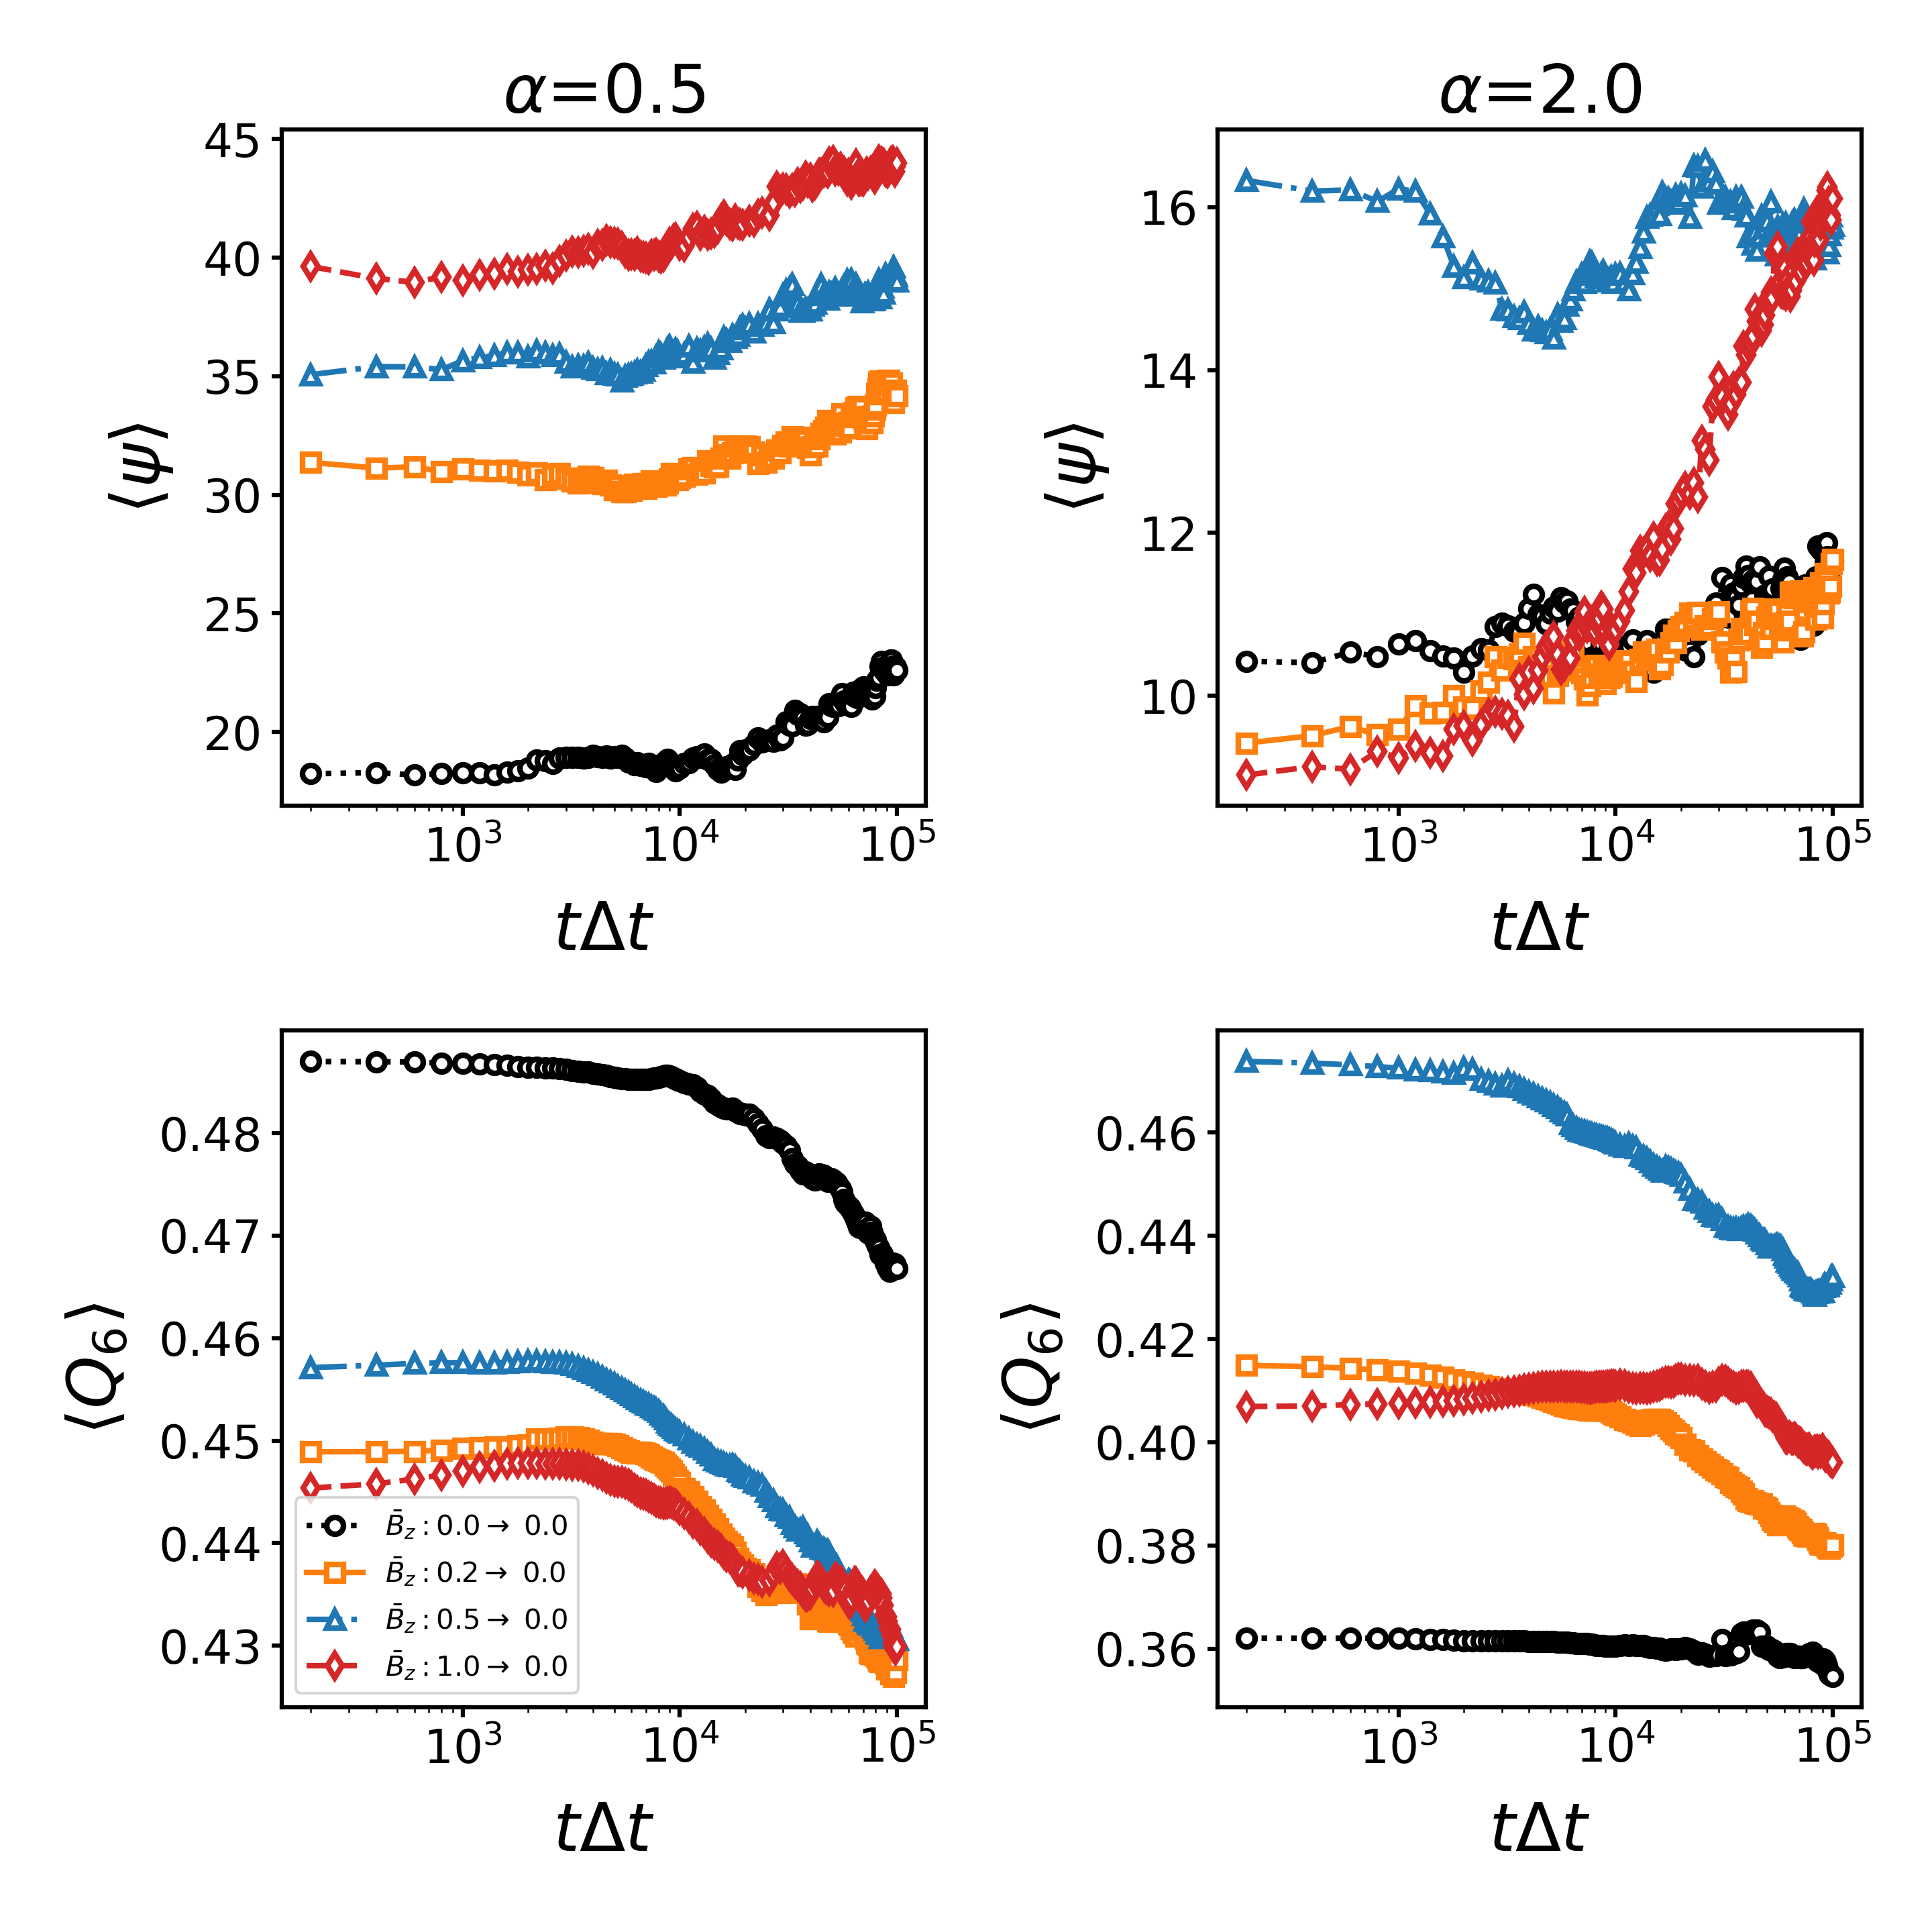
\includegraphics[scale=0.4]{../figures/results/paper2/interface_angle-nint-field_down.png} 
\caption{Plots of the average interfacial angle $\psi$ and the number of particles on the interface $n_{int}$ on the left and right respectively, plotted against time for bijels stabilized with ellipsoidal particles with aspect ratio 2. When looking at $\psi$, the $\bar{B}:1 \rightarrow 1$ case looks distinctly different from the other processes. At $\bar{B} = 1$, the particles are totally ordered to the field. This suggests that the presence of some particle disorder resists domain coarsening.} 
\label{fig:interface_angle-field_down} 
\end{figure}

In Figure \ref{fig:interface_angle-field_down}, we plot
\(\langle \psi \rangle\) and \(\langle Q_6 \rangle\) in the left and
right columns respectively. While there are minor differences to the
time when \(\langle \psi \rangle\) and \(\langle Q_6 \rangle\) increase
and decrease respectively for bijels stabilized by oblate particles the
trends are identical. This suggests that the differences in particle
angle, local ordering and nematic order only change when coarsening will
take place without affecting its dynamics.

For prolate particles, we see that a reduction in
\(\langle \psi \rangle\) takes place for all runs except for
\(\bar{B}: 0.5\rightarrow 0\). This is attributed to be due to this
system being near its preferred interface angle, with changes occurring
as the particles reorient away from the magnetic field causing
deviations before returning to that angle. We see that the
\(\bar{B}: 1\rightarrow 0\) case also reaches approximately the same
value for \(\langle \psi \rangle\). \(\bar{B}: 0.2\rightarrow 0\) and
\(\bar{B}: 0\rightarrow 0\) reduce much more slowly than
\(\bar{B}: 1\rightarrow 0\). This suggests that local reorientation is
occurring, although its affects manifest as insignificant changes in the
microstructure of the material.

Looking at \(\langle Q_6 \rangle\), we see that all simulations see a
decrease over time. We see that contrary to previous trends, the
\(\bar{B}: 1\rightarrow 0\) simulation has a smaller change in
\(\langle Q_6 \rangle\) than \(\bar{B}: 0.5\rightarrow 0\) although this
difference is also a result of the initial particle orientation and
position, rather than a defining feature of a broader trend. We see that
the \(\bar{B}: 0.5\rightarrow 0\) case is near the
\(Q_6^{HCP} \approx 0.485\) boundary, suggesting it is most susceptible
to lose short range order upon removal of the magnetic field that
enforces it, resulting in the large decrease in \(\langle Q_6 \rangle\)
observed.

We see from the microstructure evolution that steric effects are the
driving force behind microstructure changes in the absence of a magnetic
field. Even though we observe that the interface angle and Steinhardt
order parameter show substantial changes from the scenario where no
field is applied, these are insufficient to change the average steric
effect driven particle monolayer rearrangement observed, causing
coarsening of the bijel at long timescales similar what was observed by
Gunther et al.~\cite{gunther_timescales_2014}
